\chapter{Positive displacement pumps}
/note{added from Volumetric Pumps and Compressors}

\section{Introduction}

\subsection{Pumps - general introduction}

A pump is a machine that moves fluids (mostly liquids) by mechanical action. Pumps can be classified into three major groups according to the method they use to move the fluid: 
\begin{description}
\item[Centrifugal pumps] are used to transport fluids by the conversion of rotational kinetic energy to the hydrodynamic energy of the fluid flow. The rotational energy typically comes from an engine or electric motor. The fluid enters the pump impeller along or near to the rotating axis and is accelerated by the impeller. Common uses include water, sewage, petroleum and petrochemical pumping. 

\item[Positive displacement pumps] have an expanding cavity on the suction side and a decreasing cavity on the discharge side. Liquid flows into the pumps as the cavity on the suction side expands and the liquid flows out of the discharge as the cavity collapses. The volume is constant given each cycle of operation.

\item[Miscellaneous pumps] are the rest of the pumps, such as Eductor-jet pump, airlift pump, etc.
\end{description}

Pumps operate by some mechanism (typically reciprocating or rotary), and consume energy to perform mechanical work by moving the fluid. Pumps operate via many energy sources, including manual operation, electricity, engines, or wind power, come in many sizes, from microscopic for use in medical applications to large industrial pumps.

\begin{figure}[h]
\begin{center}
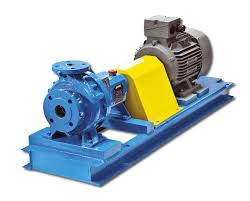
\includegraphics[width=0.4\textwidth]{pump1.jpg}
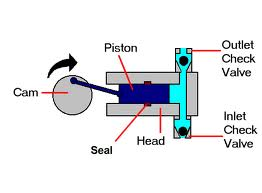
\includegraphics[width=0.45\textwidth]{rec_pump1.jpg}
\caption{\label{fig:pumps}Two examples of pumps: (left) centrifugal pump (right) positive displacement pump (piston pump)}
\end{center}
\end{figure}

Mechanical pumps serve in a wide range of applications such as pumping water from wells, aquarium filtering, pond filtering and aeration, in the car industry for water-cooling and fuel injection, in the energy industry for pumping oil and natural gas or for operating cooling towers. In the medical industry, pumps are used for biochemical processes in developing and manufacturing medicine, and as artificial replacements for body parts, e.g. the artificial heart.

The two most important quantities characterizing a pump are the pressure difference between the suction and pressure side of the pump $\Delta p$ and the flow rate delivered by the pump $Q$. For practical reasons, in the case of water technology, the \emph{pressure head} is usually used, which is pressure given in meters of fluid column: $H=\frac{\Delta p}{\rho g}$. Simple calculations reveals that for water 1 bar ($10^5\mathrm{Pa}$) pressure is equivalent of 10 mwc (meters of water column).

\subsubsection{Turbopumps}

In the case of a turbopump, a rotating impeller adds energy to the fluid. The head is computed with the help of Euler's turbine equation
%
\begin{equation}
H = \left.\frac{c_{\mathrm{2u}}u_\mathrm{2}-c_{\mathrm{1u}}u_\mathrm{1}}{g}\right|_{c_{1u=0}} =\frac{c_{\mathrm{2u}}u_\mathrm{2}}{g}
\end{equation}
%
\noindent while the flow rate is 
%
\begin{equation}
Q = D_2 \pi b_2 c_{\mathrm{2m}},
\end{equation}
%
with $c_{2u}$ and $c_{1u}$ being the circumferential component of the absolute velocity at the outlet and inlet, respectively, $u_1=D_1 \pi n$ and $u_2=D_2 \pi n$ the circumferential velocities. $c_{2m}$ stands for the radial (meridian) component of the absolute velocity at the outlet, $D$ is diameter and $b$ stand for the width of the impeller. (See Figure \ref{fig:vel_triang} and \emph{Fluid Machinery} lecture notes for further details.)

\begin{figure}[h]
\begin{center}
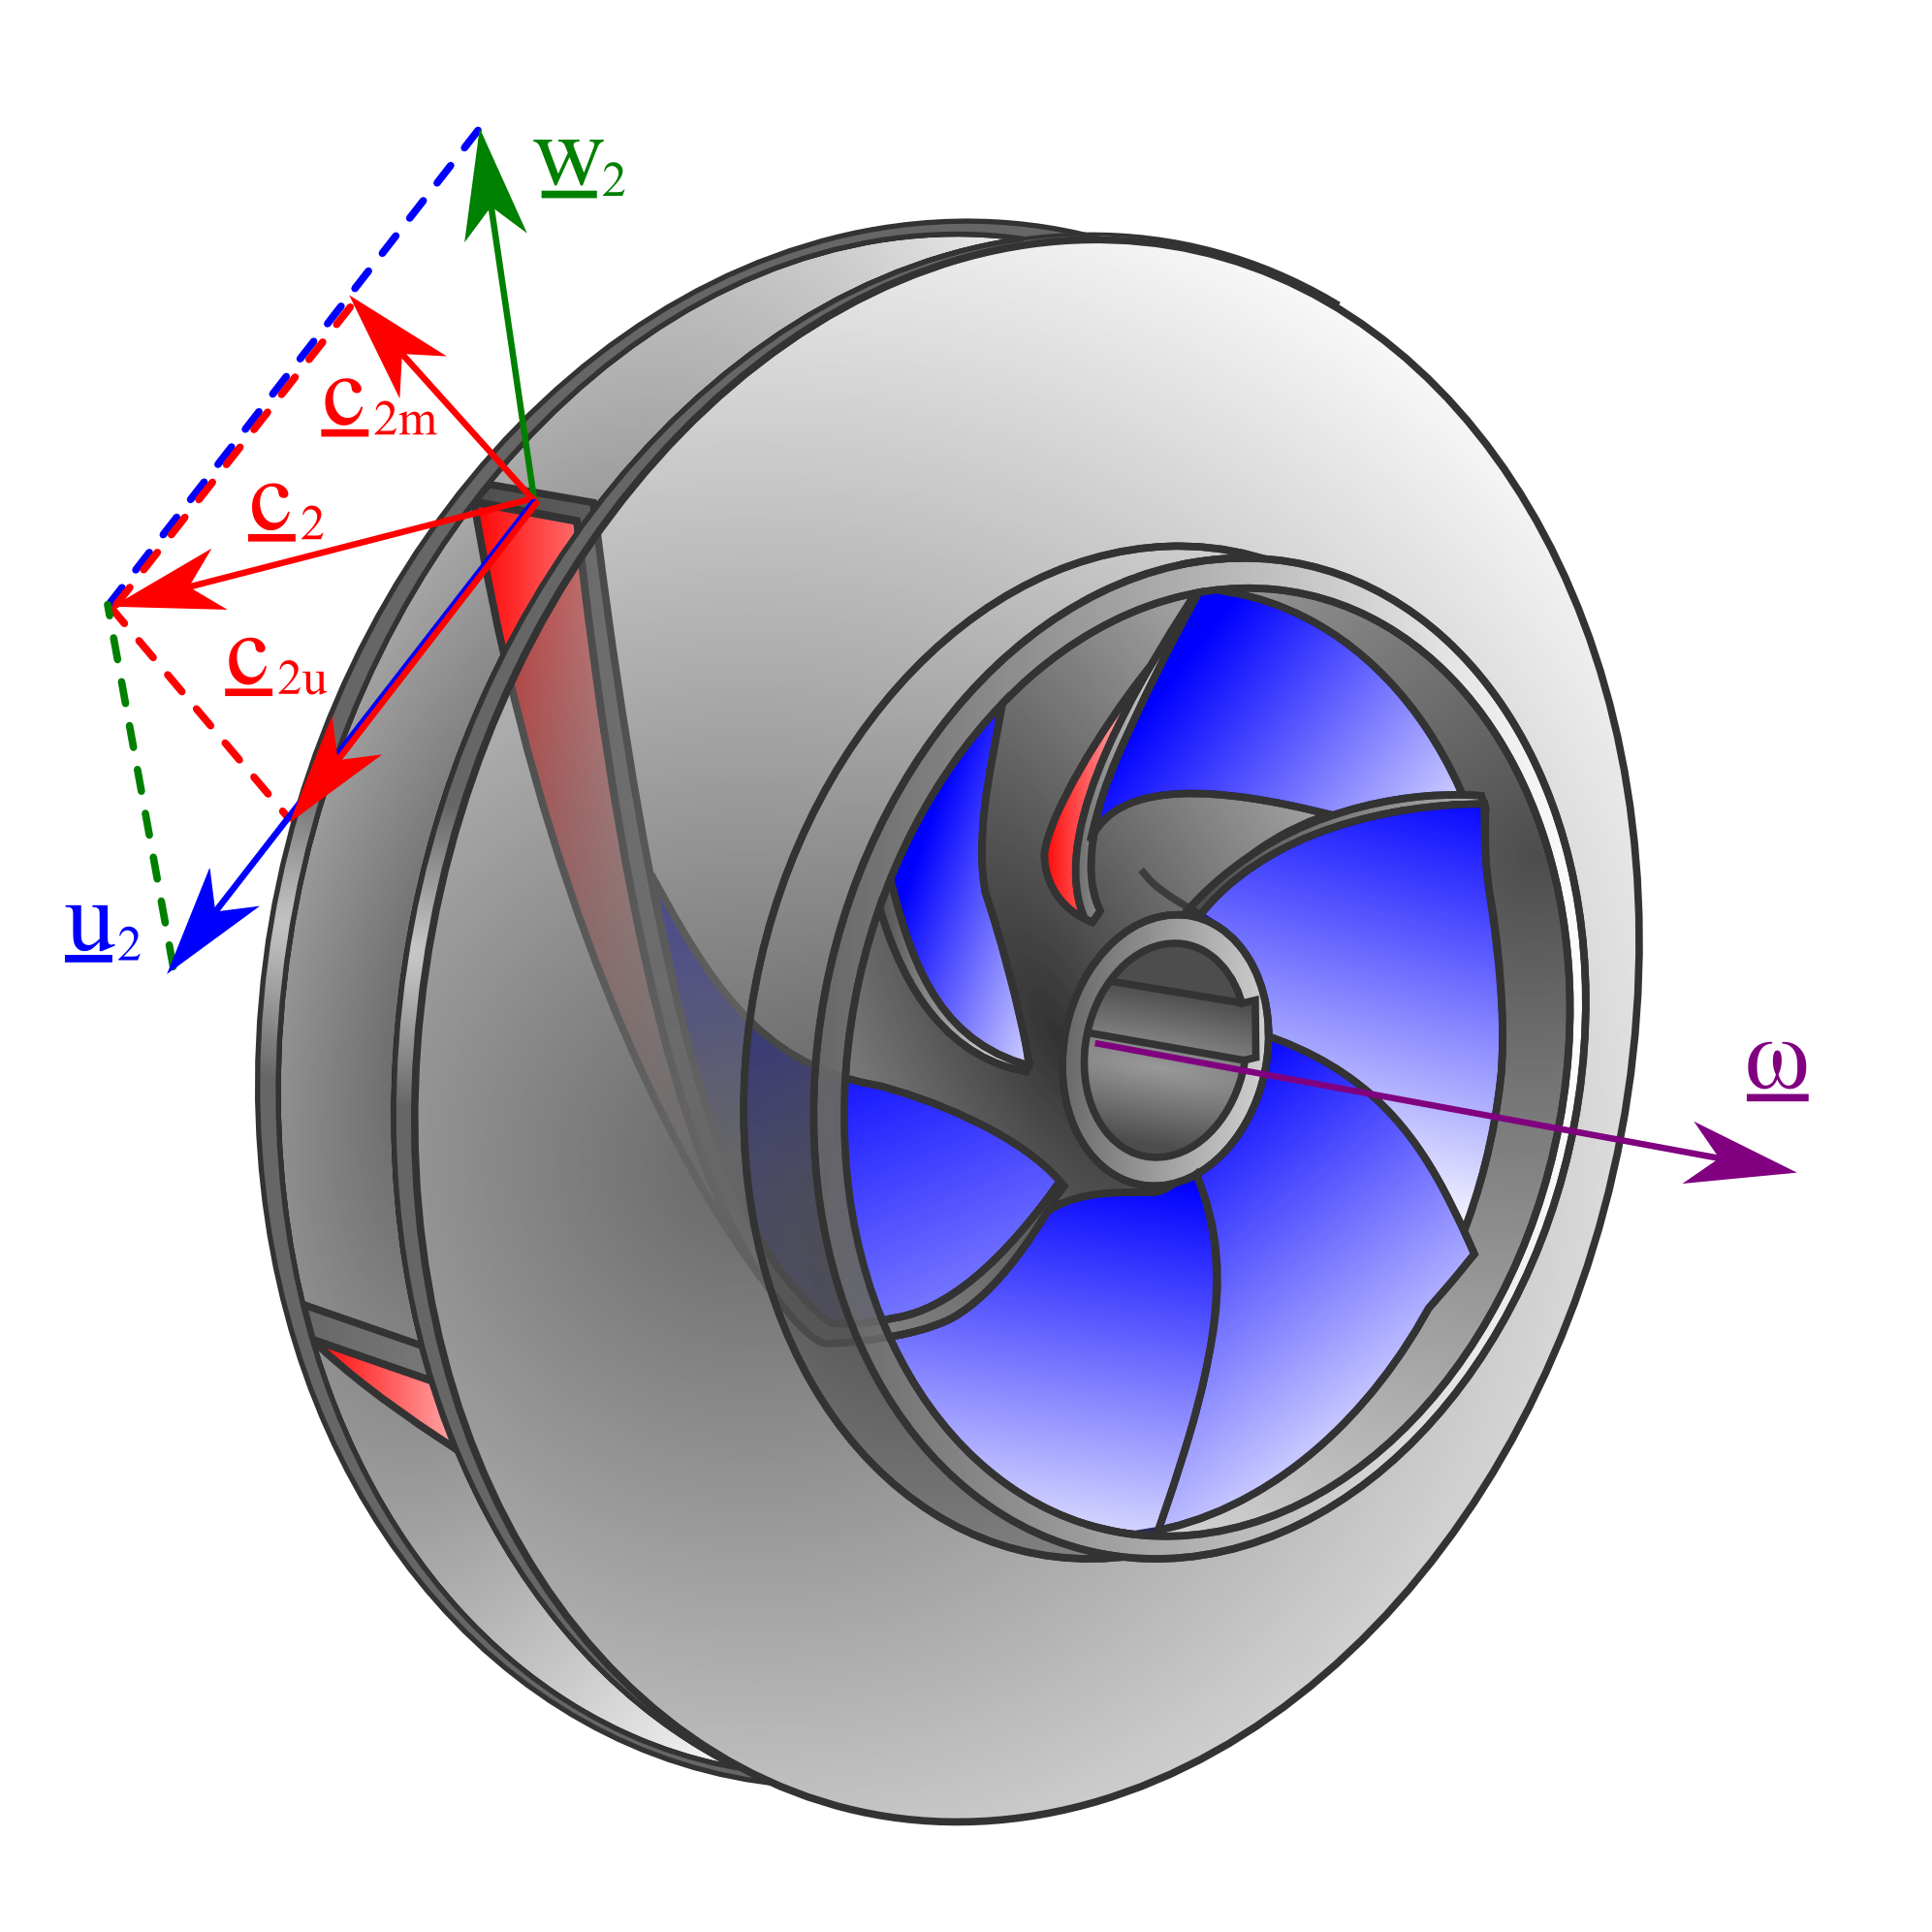
\includegraphics[width=0.4\textwidth]{Impeller3D_and_VelocityTriangles.png}
\caption{\label{fig:vel_triang}Velocity triangles on a centrifugal impeller.}
\end{center}
\end{figure}

Notice that the head ($H$) and flow rate ($Q$) are provided by the two component of the same velocity vector $c_2$. Thus, if $H$ increases, $Q$ decreases and vice versa. Thus \emph{in the case of turbomachines the pressure difference and the flow rate are directly connected and not independent.} This dependency is described by the pump's performance curve, see Figure \ref{fig:turbopump_perf_curve}.

\begin{figure}[th]
\begin{center}
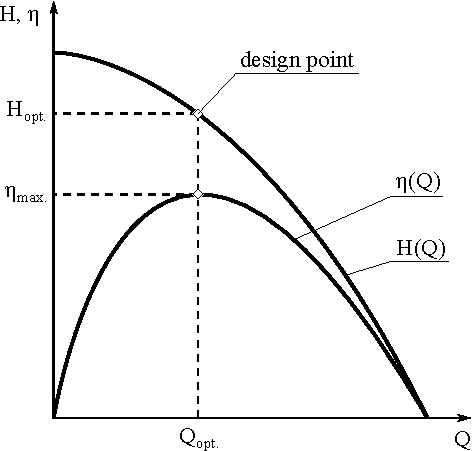
\includegraphics[scale=0.8]{lecture1_fig01_QH.pdf}
\caption{\label{fig:turbopump_perf_curve}Turbopump performance curves}
\end{center}
\end{figure}

An important quantity describing the shape of the impeller of a turbopump is the specific speed $n_q$, defined as
%
\begin{equation}
n_q=n\,\frac{Q^{1/2}_{\mathrm{opt.}}}{H^{3/4}_{\mathrm{opt.}}}\quad \mathrm{[rpm]}\,\frac{\mathrm{[m^3/s]^{1/2}}}{\mathrm{[m]^{3/4}}}.
\end{equation}
%
The dimension (unit) of $n_q$ is not emphasised and mostly omitted. The concept of specific speed can be used to determine the pump type (i.e. radial/mixed/axial) which is capable of performing a pumping problem efficiently.

\begin{figure}[h!]
\begin{center}
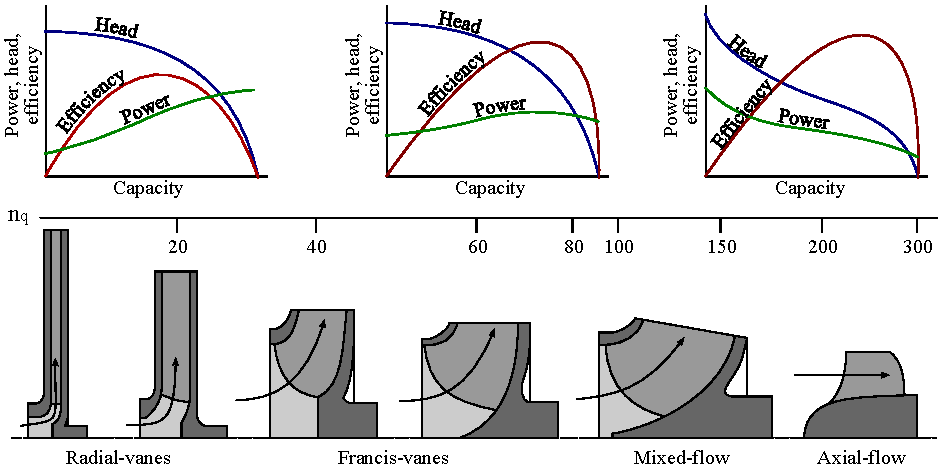
\includegraphics[scale=0.8]{nq.pdf}
\caption{\label{fig:nq}Turbopump performance curves}
\end{center}
\end{figure}

%%%%%%%%%%%%

\vspace{0.5cm}

\noindent {\bf Example 1.} We have to pump clean water to an upper reservoir at 60 m height. The nominal power of the driving electric motor is 5 kW, its revolution number is 3000 rpm. The flow rate is (assuming 100\% efficiency)
%
\begin{equation}
P_{\mathrm{motor}}=\Delta p\cdot Q\rightarrow Q=\frac{P_{\mathrm{motor}}}{\Delta p}=\frac{P_{\mathrm{motor}}}{\rho gH}=8.49\times 10^{-3}\,\mathrm{m^3/s}=509\,\mathrm{l/min}
\end{equation}
%
\noindent Hence the specific speed is
%
\begin{equation}
n_q=n\,\frac{Q^{1/2}_{\mathrm{opt.}}}{H^{3/4}_{\mathrm{opt.}}}=3000\frac{\left(8.49\times 10^{-3}\right)^{1/2}}{\left(60\right)^{3/4}}\cong 12.8,
\end{equation}
%
\noindent which means that a centrifugal turbopump is suitable for this problem.

%%%%%%%%%%%%

\vspace{0.5cm}

\noindent {\bf Example 2.} Now consider the hydraulic cylinder depicted in Figure \ref{fig:hydraulic_cylinder}. The required pressure difference is now $\Delta p=200 \mathrm{bar} = 2\times 10^7 \mathrm{Pa}$, the power and the revolution number of the driving motor is the same as before (5kW, 3000rpm).

\begin{figure}[tbh]
\begin{center}
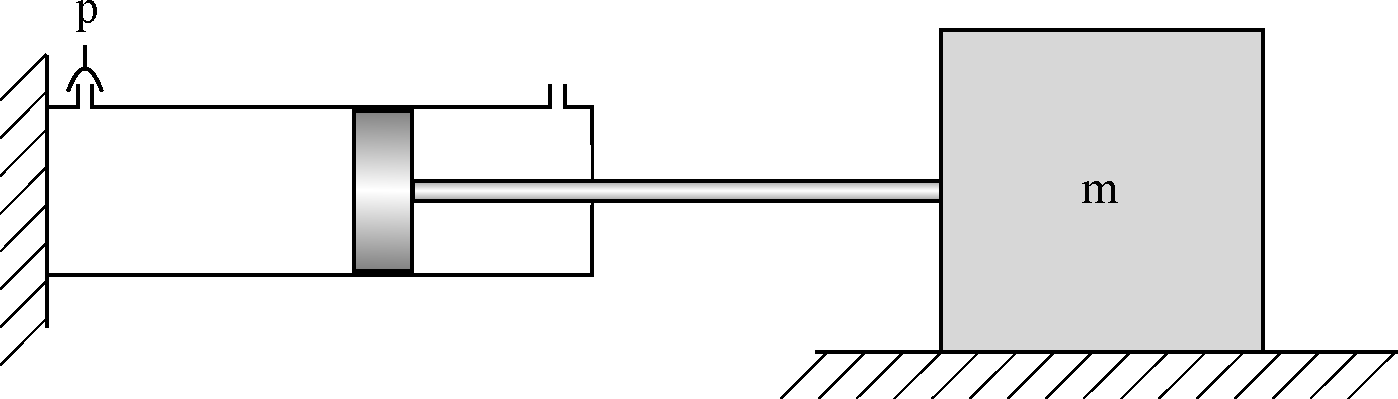
\includegraphics[width=100mm]{lecture1_fig02_dugattyu.pdf}
\caption{\label{fig:hydraulic_cylinder}Simple sketch of a hydraulic cylinder}
\end{center}
\end{figure}

\noindent First, find the flow rate of the pump (again, assume 100\% efficiency):
%
\begin{equation}
Q=\frac{P_{\mathrm{motor}}}{\rho gH}=\frac{5000}{9810\cdot 2000}=2.55\times 10^{-4}\,\mathrm{m^3/s}=15.3\,\mathrm{liter/min},
\end{equation}
%
which gives
%
\begin{equation}
n_q=n\,\frac{Q^{1/2}_{\mathrm{opt.}}}{H^{3/4}_{\mathrm{opt.}}}=3000\frac{\left(2.55\times 10^{-4}\right)^{1/2}}{\left(2000\right)^{3/4}}= 0.16.
\end{equation}
%
\noindent Comparing this value with Figure \ref{fig:nq} we see that this value is 'off' the chart. Such a small $n_q$ value would require an extremely large-diameter impeller, which is very thin. Besides the problems with the high centrifugal stresses, from the fluid mechanical point of view, such a thin impeller introduces extremely large fluid friction resulting in poor efficiency. Thus we conclude that {\bf pumping problems resulting in high pressure difference and low flow rates (i.e. $n_q< \mathrm{say,} 10$) cannot be efficiently solved by centrifugal pumps}.


\subsubsection{Positive displacement pumps}

Positive displacement pumps (PDPs) are typically used in high-pressure (above $\Delta p > 10 bar$, up to 1000-2000 bars) technology, with relatively low flow rate. These machines have an expanding cavity on the suction side and a decreasing cavity on the discharge side. Liquid flows into the pumps as the cavity on the suction side expands and the liquid flows out of the discharge as the cavity collapses. The volume is constant given each cycle of operation.

The positive displacement pumps can be divided in two main classes (see Figures XXX)
\begin{itemize}
\item reciprocating
\begin{itemize}
\item piston pumps
\item plunger pumps
\item diaphragm pumps
\item axial/radial piston pumps
\end{itemize}
\item rotary
\begin{itemize}
\item gear pumps
\item lobe pumps
\item vane pumps
\item progressive cavity pumps
\item peripheral pumps
\item screw pumps
\end{itemize}
\end{itemize}

\begin{figure}[h!]
\begin{center}
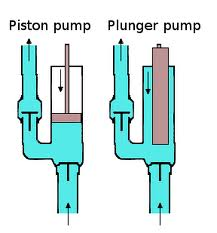
\includegraphics[width=0.3 \textwidth]{plunger_piston_pump.jpg}
\includegraphics[width=0.45 \textwidth]{axial_piston_pump.jpg}
\caption{\label{fig:reiprocating_pumps}Some reciprocating pumps}
\end{center}
\end{figure}

\begin{figure}[h!]
\begin{center}
\includegraphics[width=0.3 \textwidth]{gear_pump.jpg}
\includegraphics[width=0.3 \textwidth]{vane_pump.jpg}
\includegraphics[width=0.3 \textwidth]{double-screw_pump.jpg}
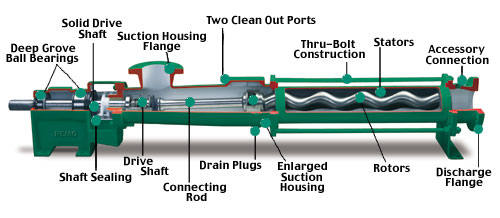
\includegraphics[width=0.6 \textwidth]{progressive_cavity_pump.jpg}
\caption{\label{fig:reiprocating_pumps}Some rotary pumps}
\end{center}
\end{figure}

PDPs, unlike a centrifugal pumps, will produce the same flow at a given motor speed (rpm) no matter the discharge pressure, hence PDPs are \emph{constant flow machines}. A PDP must not be operated against a closed valve on the discharge (pressure) side of the pump because it has no shut-off head like centrifugal pumps: a PDP operating against a closed discharge valve will continue to produce flow until the pressure in the discharge line are increased until the line bursts or the pump is severely damaged - or both.

A relief or safety valve on the discharge side of the PDP is therefore absolute necessary. The relief valve can be internal or external. The pump manufacturer has normally the option to supply internal relief or safety valves. The internal valve should in general only be used as a safety precaution, an external relief valve installed in the discharge line with a return line back to the suction line or supply tank is recommended.

Several types of PDPs can be used as motors: if fluid is driven through them (e.g. gear pump), the shaft rotates and the same machine can be used as a motor.

\clearpage

\subsection{Basic characteristics of positive displacement machines} \label{sec:basic_characteristics_of_positive_displacement_machines}

The pump \emph{displacement} $V_g$ is the volume of the liquid delivered by the pump per one revolution, assuming no leakage (zero pressure difference between the suction and pressure side) and neglecting the fluid compressibility. The \emph{ideal -- theoretical -- flow rate} is
%
\begin{equation}
Q_{th}=n V_g
\label{eq:Qth}
\end{equation}
%
where $Q_{th}$ is theoretical flow rate ($\mathrm{liter/min})$, $n$ is the revolution number of the pump shaft ($\mathrm{rpm}$) and $V_g$ stands for the pump displacement, ($\mathrm{cm^3}$). 

In the case of {\bf pumps}, the actual outflow is less than the theoretical flow rate, due to the leakages inside the pump. These losses are taken into by the \emph{volumetric efficiency} $\eta_{vol}$: $Q=\eta_{\mathrm{vol}} Q_{\mathrm{th}} = \eta_{\mathrm{vol}}\, n\,  V_{\mathrm{g}}$. Other types of losses (sealing, bearing, fluid internal and wall friction) are all concentrated into the so-called \emph{hydromechanical efficiency} $\eta_{hm}$, which connects the input and output power: $P_{in} \eta_{hm}=P_{out}$. For pumps, $P_{in}=M \omega$ and $P_{out}=Q \Delta p$. We have:
%
\begin{equation} \label{power_balance_of_positive_displacement_machines}
\eta_{hm} \underbrace{M \underbrace{2\pi n}_{\omega}}_{P_{in}}=\underbrace{\underbrace{n V_g \eta_{vol}}_Q\Delta p}_{P_{out}}
\quad \rightarrow \quad
\Delta p_{pump}=\frac{2\pi M}{V_{\mathrm{g}}}\frac{\eta_{hm}}{\eta_{vol}}
\end{equation}

In the case of {\bf motors}, the input power is hydraulic power ($P_{in}=Q \Delta p$) and the output is rotating mechanical power $P_{out}=M \omega$. Due to the internal leakage, one has to 'push' more fluid into the pump to experience the same revolution number, hence $Q=Q_{th}/\eta_{vol}>Q_{th}$. We have:
%
\begin{equation}
\eta_{hm} 
\underbrace{
\underbrace{
\frac{n V_g}{\eta_{vol}}
}_Q
\Delta p}_{P_{in}}=\underbrace{M \underbrace{2\pi n}_{\omega}}_{P_{out}}
\quad \rightarrow \quad
\Delta p_{motor}=\frac{2\pi M}{V_{\mathrm{g}}}\frac{\eta_{vol}}{\eta_{hm}}
\end{equation}

\begin{figure}[ht]
\begin{center}
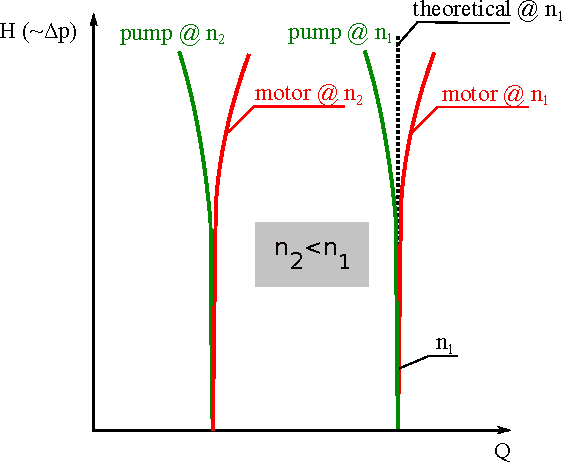
\includegraphics[width=0.5 \textwidth]{motor_pump_perf_curve_QH.pdf}
\caption{\label{fig:pump_and_motor_perf_curve}Pump and motor performance curves for two different revolution mubers.}
\end{center}
\end{figure}

\noindent We conclude that for both pumps and motors,

\begin{equation}
\shadowbox{$\displaystyle
Q \propto n,V_g \quad \text{and} \quad \Delta p \propto M,\frac{1}{V_g}.
$}
\end{equation}

\noindent Which means that the pressure and the flow rate are independent for a given machine. The same behaviour can be observed on the performances curve of these machines, see Figure \ref{fig:pump_and_motor_perf_curve}. The theoetical performance lines are vertical for a given revolution speed, meaning that the theoretical flow rate does not change when varying the pressure.

However, the leakage flow rate through the small internal gaps of the pumps (motors) slighty change ths theoretical behaviour. In the case of pumps, a portion of the flow rate flows back from the pressure side to the suction side through these gaps, hence reducing the outflow of the pump. The higher the pressure difference is, the higher the leakage flow rate is, hence the pump performance curves tend to `bend to the left' from the vertical, theoretical line. In the case of motors, where the fluid drives the shaft, we need larger flow rates to reach the desired revolution number, hence the real curves `bend to the right'.

\clearpage

\section{Reciprocating Pumps}

Piston/plunger pumps comprise of a cylinder with a reciprocating piston/plunger in it. In the head of the cylinder the suction and discharge valves are mounted. In the suction stroke the plunger retracts and the suction valves opens causing suction of fluid into the cylinder. In the forward stroke the plunger push the liquid out the discharge valve.

With only one cylinder the fluid flow varies between maximum flow when the plunger moves through the middle positions, and zero flow when the plunger is in the end positions. A lot of energy is wasted when the fluid is accelerated in the piping system. Vibration and "water hammers" may be a serious problem. In general the problems are compensated by using two or more cylinders not working in phase with each other.

Several cylinders can be mounted to the same shaft: pumps with 1 cylinder are called \emph{simplex} pumps, \emph{duplex} pumps have two cylinders (with $\pi$ phase shift) while \emph{triplex} pumps have three pumps with $2 \pi/3 = 120$ degrees phase shift. Pumps with even more pistons (5,7,9) are also common. Pumps with both sides of the piston acting (deing in contact with the liquied) are called \emph{double-acting} pumps.


\subsection{Single-acting piston pumps}




\begin{figure}[tbh]
\begin{center}
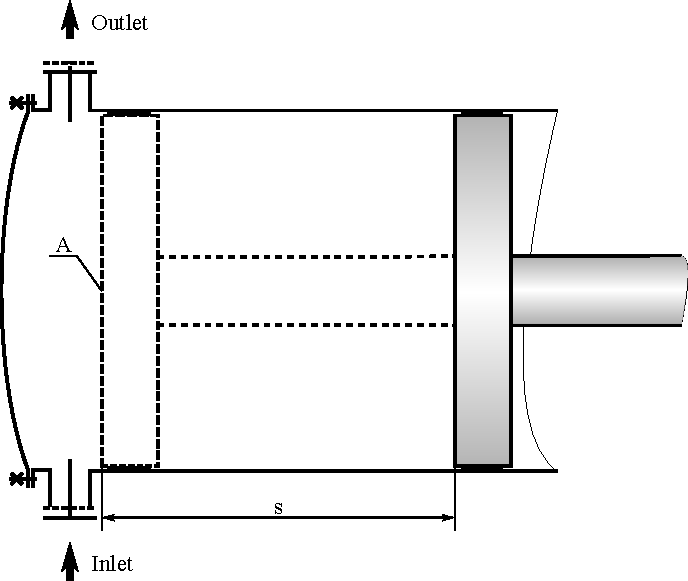
\includegraphics[scale=0.7]{lecture2_fig10_dugattyus_szivattyu.pdf}
\caption{\label{fig:single_acting_piston_pump}Single-acting piston pump}
\end{center}
\end{figure}

Consider the piston pump depicted in Figure \ref{fig:single_acting_piston_pump}.  First, let us find the $x(t)$ displacement of the piston as a function of time. By virtue of the cosine law, we have
%
\begin{equation}
L^2=R^2+y(t)^2- 2 R y(t) \cos \varphi \quad \rightarrow \quad y(t)=R \cos \varphi \pm \sqrt{L^2+R^2\left( 1-\cos^2 \varphi\right)}
\end{equation}
%
with $\varphi=\omega t$. Notice that if $\varphi=0$, we must have $y(0)=R+L$, hence we need the 'plus' case in the above equation. The piston displacement is 
%
\begin{equation}
x(t)=y(t)-y(\pi)=R \left( 1+ \cos \varphi  - \lambda^{-1} \left(
1- \sqrt{1+\lambda^2\left( 1-\cos^2 \varphi\right)}
\right)\right),
\end{equation}
%
with $\lambda=R/L$. Now consider the terms in the bracket. First, $1+\cos \varphi$ varies between 0 and 2. The second term varies between 0 ($\cos \varphi=\pm1$) and $\lambda^{-1} \left(1- \sqrt{1+\lambda^2} \right)$ ($\cos \varphi=0$), which gives $0.2361$, $0.099$ and $0.0499$ for $\lambda=R/L=1/2,1/5$ and $1/10$, respectively. Hence we conclude that if $\lambda<0.2$ (which s trus for many real-life configurations), the error due to neglecting the $\lambda^{-1}(\dots)$ term is less than 10\%, which is acceptable.

Hence we approximate the piston displacement as
%
\begin{equation}
x(t)\approx R\left(1+\cos \left( \omega t\right) \right), \quad 
v(t)\approx-R \omega \sin \left( \omega t\right) \quad \text{and} \quad 
a(t)\approx-R \omega^2 \cos \left( \omega t\right).
\end{equation}
%
As flow rate is $Q=Av$ and the stroke is $s=2R$, the \emph{instantaneous} pressure side flow rate is (see also Figure \ref{fig:single_acting_piston_pump_curves})
%
\begin{equation}
Q(t)=
\begin{cases}
A\frac{s}{2}\omega\cos(\omega t) & \mathrm{if} \quad  \pi < \varphi=\omega t < 2 \pi \\
0 & \mathrm{if}\quad  0 < \varphi=\omega t < \pi
\end{cases}
\label{eq:single_piston_pump_flowrate}
\end{equation}
% \begin{equation}
% Q(t)=A\underbrace{v(t)}_{\frac{\mathrm{d}}{\mathrm{d}t}x(t)}=A\frac{s}{2}\omega\cos(\omega t).
% \label{eq:single_piston_pump_flowrate}
% \end{equation}
%
The mean flow rate is computed by finding the volume of the fluid pushed to the pressure side in one period, divided by the length of the period:
%
\begin{equation}
Q_{mean} = A s n, 
\end{equation}
%
that is, we have $V_g = A s$, see \eqref{eq:Qth}. The maximum flow rate is (see \eqref{eq:single_piston_pump_flowrate})
%
\begin{equation}
Q_{max} = A \frac{s}{2} \omega= \pi A s n = \pi Q_{mean}. 
\end{equation}

\begin{figure}[th]
\begin{center}
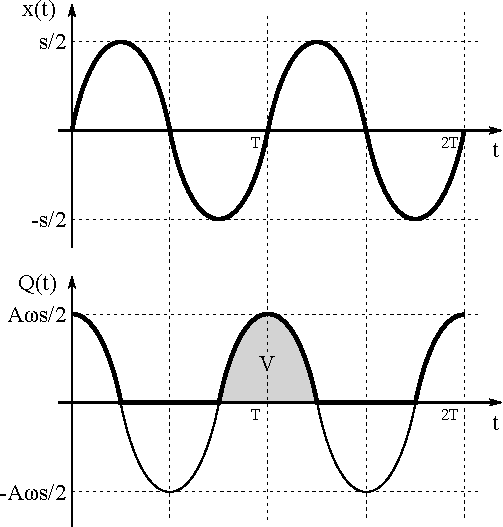
\includegraphics[width=0.5\textwidth]{lecture2_fig11_dugattyus_szivattyu_diagram.pdf}
\caption{\label{fig:single_acting_piston_pump_curves} Piston displacement (upper panel) and flow rate ($\propto$ velocity) curves of a single-acting piston pump.}
\end{center}
\end{figure}

Notice that this means that these pumps induce an extremely unsteady flow rate in the pipeline system, that varies from $Q_{min}=0$ flow rate up to $Q_{max}=\pi Q_{mean}$ with a frequency of $n$ (driving motor revolution number). There are two ways of reducing this pulsation: (a) by using multiple pistons or (b) adding a pulsation damper.

\clearpage

\subsection{Multiple piston pumps}

The pulsation can be reduced by adding several pistons with an evenly distributed phase shift, see e.g. Figure \ref{fig:double_acting_piston_pump}. 

\begin{figure}[th]
\begin{center}
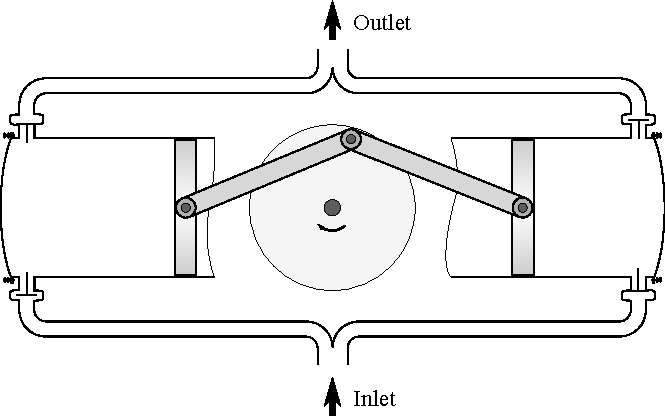
\includegraphics[scale=0.9]{lecture2_fig12_duplex_dugattyus_szivattyu.pdf}
\caption{\label{fig:double_acting_piston_pump}Double-acting piston pump}
\end{center}
\end{figure}

\noindent If we have three pistons (triplex), the flow rates are 
%
\begin{align*}
Q_1(t) &= \text{max}(0, A s n \pi\cos(\omega t))\\
Q_2(t) &= \text{max}(0, A s n \pi\cos(\omega t-\frac{2\pi}{3}))\quad \text{and}\\
Q_3(t) &= \text{max}(0, A s n \pi\cos(\omega t-2 \times\frac{2\pi}{3})).
\end{align*}
%
The overall flow rate is $Q(t)=Q_1(t)+Q_2(t)+Q_3(t)$. Let us define the \emph{pulsation factor} measuring the relative flow rate change as
%
\begin{equation}
\delta =\frac{Q_{\mathrm{max}}-Q_{\mathrm{min}}}{Q_{\mathrm{mean}}}\,[\%].
\end{equation}
%
For example, for a single-acting pump we have
\begin{equation}
\delta =\frac{Q_{\mathrm{max}}-Q_{\mathrm{min}}}{Q_{\mathrm{mean}}}=\frac{\pi Q_{\mathrm{mean}}-0}{Q_{\mathrm{mean}}}=\pi = 314\,\%
\end{equation}

\begin{figure}[ht]
\begin{center}
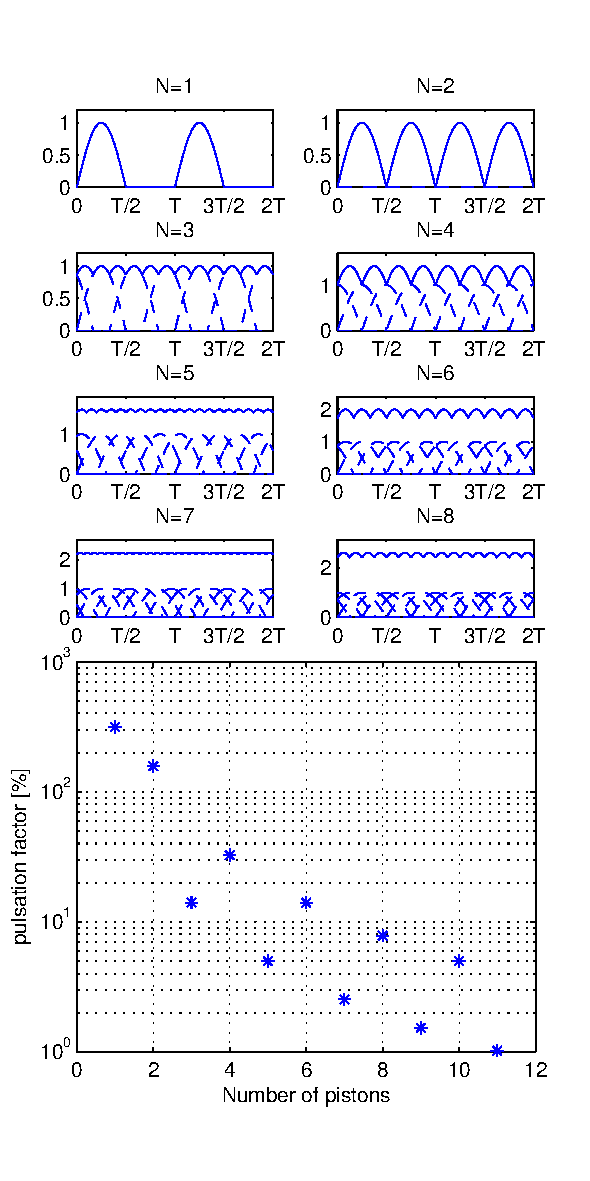
\includegraphics[width=12cm]{piston_pump_pulsation_factor.pdf}
\caption{\label{fig:pulsation_factor}Pulsation factor as a function of the piston number.}
\end{center}
\end{figure}

Similar calculation for other number of pistons gives the values in Table \ref{tab:piston_puls}. Figure \ref{fig:pulsation_factor} depicts the flow rate for several numbers of pistons, where dashed lines are the individual flow rates while solid lines are the pump flow rate (sum of the piston flow rates) and the pulsation factor as a function of the piston number. Notice that if the number of pistons is odd (e.g. 3,5,7,9), the pulsation number is significantly lower.

\begin{table}[h]
\centering
\begin{tabular}{l||c|c|c|c|c|c|}
Number of pistons & 1 & 2 & 3 & 4 & 5 & 9\\ \hline
$\delta $ \%      &  315 & 157 & 14 & 33 & 5 & 1.5
\end{tabular}
\caption{\label{tab:piston_puls}Flow rate pulsation level as a function of the piston number.}
\end{table}
\clearpage

%%%%%%%%%%%%%%%%%%%%%%%%%%%%%%%%%%%%%%%%%%%%%%%%%%%%
\subsection{Axial piston pumps}

An axial piston pump is a positive displacement pump that has a number of pistons in a \emph{circular array} within a cylinder block. It can be used as a stand-alone pump, a hydraulic motor or an automotive air conditioning compressor. Axial piston pumps are used to power the hydraulic systems of jet aircrafts, being gear-driven off of the turbine engine's main shaft. The system used on the F-14 used a 9-piston pump that produced a standard system operating pressure of 3000 psi and a maximum flow of 84 gallons per minute.  Advantages:

\begin{itemize}
\item high efficiency
\item  high pressure (up to 1,000 bar)
\item  low flow and pressure ripple (due to the small dead volume in the workspace of the pumping piston)
\item low noise level
\item high reliability
\end{itemize}


Axial piston units are available in the form of pumps and motors in bent axis design or swashplate design for medium- and high-pressure ranges. They are the main components in the hydrostatic transmission. Compact size and high power density, economy and reliability are characteristic advantages which speak for the use of hydrostatic transmissions, together with the fact that they meet the demand for high speed and high torque, as well as optimum efficiency. 

\begin{figure}[h!]
\begin{center}
\includegraphics[height=5cm]{figs/axial_piston_pump.jpg}
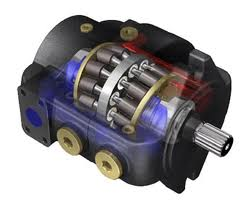
\includegraphics[height=5cm]{figs/axial_piston_pump_cutaway.jpg}
\caption{\label{fig:ax_pp} Axial piston pump}
\end{center}
\end{figure}

%%%%%%%%%%%%%%%%%%%%%%%%%%%%%%%%%%%%%%%%%%%%%%%%%%%%
\subsection{Radial piston pumps}

In a radial piston pump the working pistons extend in a radial direction symmetrically around the drive shaft, in contrast to the axial piston pump. These kinds of piston pumps are characterized by the following advantages:
\begin{itemize}
\item high efficiency
\item  high pressure (up to 1,000 bar)
\item  low flow and pressure ripple (due to the small dead volume in the workspace of the pumping piston)
\item low noise level
\item very high load at lowest speed due to the hydrostatically balanced parts possible
\item no axial internal forces at the drive shaft bearing
\item high reliability
\end{itemize}

A disadvantage are the bigger radial dimensions in comparison to the axial piston pump, but it could be compensated with the shorter construction in axial direction.

Due to the hydrostatically balanced parts it is possible to use the pump with various hydraulic fluids like mineral oil, biodegradable oil, HFA (oil in water), HFC (water-glycol), HFD (synthetic ester) or cutting emulsion. That implies the following main applications for a radial piston pump:
machine tools (e.g., displace of cutting emulsion, supply for hydraulic equipment like cylinders)
\begin{itemize}
\item high pressure units (HPU) (e.g., for overload protection of presses)
\item test rigs
\item automotive sector (e.g., automatic transmission, hydraulic suspension control in upper-class cars)
\item plastic- and powder injection moulding
\item wind energy
\end{itemize}

\begin{figure}[h!]
\begin{center}
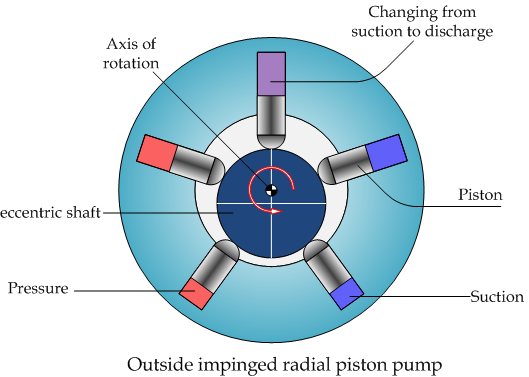
\includegraphics[height=5cm]{figs/radial_piston_pump1.png}
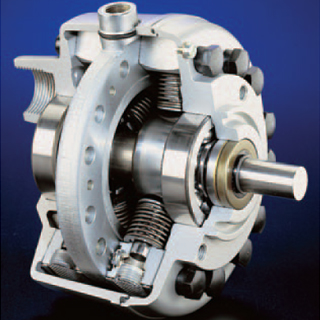
\includegraphics[height=5cm]{figs/radial_piston_pump_cutaway.jpg}
\caption{\label{fig:rad_pp} Radial piston pump}
\end{center}
\end{figure}

%%%%%%%%%%%%%%%%%%%%%%%%%%%%%%%%%%%%%%%%%%%%%%%%%%%%
\subsection{Diaphragm pumps}

A diaphragm pump (also known as a membrane pump) is a positive displacement pump that uses a combination of the reciprocating action of a rubber, thermoplastic or teflon diaphragm and suitable valves either side of the diaphragm (check valve, butterfly valves, flap valves, or any other form of shut-off valves) to pump a fluid. The advantages of these pumps are:
\begin{itemize}
\item They provide \emph{leakage-free sealing}, which can be important when pumping highly aggressive or toxic fluids.
\item They have good suction lift characteristics, some are low pressure pumps with low flow rates; others are capable of higher flow rates, dependent on the effective working diameter of the diaphragm and its stroke length. 
\item They can handle sludges and slurries with a relatively high amount of grit and solid content.
\item Suitable for discharge pressure up to 1200 bar
\item They have good dry running characteristics.
% \item can be used to make artificial hearts.
% are used to make air pumps for the filters on small fish tanks.
\item Good efficiency (can be up to 97\%)
\item Can handle highly viscous liquids.
\end{itemize}

However, as they are single (or sometimes double-acting) piston pumps, these pumps cause a pulsating flow that may cause water hammer, which can be minimised by using a pulsation dampener.

\begin{figure}[h!]
\begin{center}
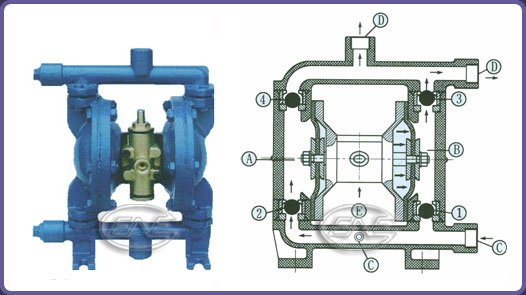
\includegraphics[width=\textwidth]{figs/diaphragmpump61_1.jpg}
% 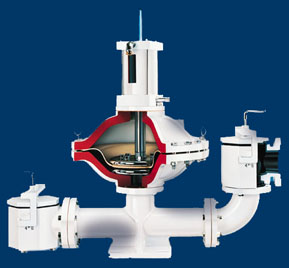
\includegraphics[height=5cm]{figs/gr-addcutaway.jpg}
\caption{\label{fig:diap_pp} Diaphragm pump}
\end{center}
\end{figure}

\clearpage

%%%%%%%%%%%%%%%%%%%%%%%%%%%%%%%%%%%%%%%%%%%%%%%%%%%%%%%%%%%%%%%%%%%%%%%%%%%%%%%%%%%%%%%%%%%%%%%%%%

\section{Rotary pumps}

\subsection{Gear pumps}
This is the simplest of rotary positive displacement pumps consisting of two meshed gears rotating in a closely fitted casing. Fluid is pumped around the outer periphery by being trapped in the tooth spaces. It does not travel back on the meshed part, since the teeth mesh closely in the centre. It is widely used on car engine oil pumps, and also in various hydraulic power packs.

There are two main variations; external gear pumps which use two external spur gears, and internal gear pumps which use an external and an internal spur gear. Some gear pumps are designed to function as either a motor or a pump.

\begin{figure}[h!]
\begin{center}
\includegraphics[height=4cm]{figs/gear_pump.jpg}
\hspace{1cm}
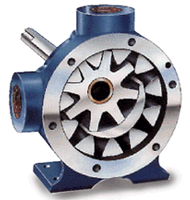
\includegraphics[height=5cm]{figs/genpur.png}
\caption{\label{fig:gear_pumps} (left) external gear pump (right) internal gear pump}
\end{center}
\end{figure}

\subsubsection{External gear pumps}

\noindent Advantages:
\begin{itemize}
\item High speed
\item High pressure
% \item No overhung bearing loads
\item Relatively quiet operation
\end{itemize}

\noindent Disadvantages:
\begin{itemize}
\item Four bushings in liquid area
\item No solids allowed
\item Fixed end clearances
\end{itemize}

\noindent Common external gear pump applications include, but are not limited to:
\begin{itemize}
\item Various fuel oils and lube oils
\item Chemical additive and polymer metering
\item Chemical mixing and blending (double pump)
\item Industrial and mobile hydraulic applications (log splitters, lifts, etc.)
\item Acids and caustic (stainless steel or composite construction)
% \item Low volume transfer or application
\end{itemize}

\subsubsection{Internal gear pumps}

\noindent Advantages:
\begin{itemize}
\item Only two moving parts
\item Only one stuffing box
\item Non-pulsating discharge
\item Excellent for high-viscosity liquids
% \item Constant and even discharge regardless of pressure conditions
\item Operates well in either directions
% \item Can be made to operate with one direction of flow with either rotation
\item Low NPSH required
\item Single adjustable end clearance
\item Easy to maintain
% \item Flexible design offers application customization
\end{itemize}

\noindent Disadvantages:
\begin{itemize}
\item Usually requires moderate speeds
\item Medium pressure limitations
\item One bearing runs in the product pumped
% \item Overhung load on shaft bearing
\end{itemize} 

\noindent Common internal gear pump applications include, but are not limited to:
\begin{itemize}
\item All varieties of fuel oil and lube oil
\item Resins and polymers
\item Alcohols and solvents
\item Asphalt, bitumen, and tar
% \item Polyurethane foam (Isocyanate and polyol)
\item Food products such as corn syrup, chocolate, and peanut butter
\item Paint, inks, and pigments
\item Soaps and surfactants
\item Glycol
\end{itemize}


\subsection{Screw pump}
Screw pumps feature two or three screws with opposing thread, that is, one screw turns clockwise, and the other counterclockwise. The screws are each mounted on shafts that run parallel to each other; the shafts also have gears on them that mesh with each other in order to turn the shafts together and keep everything in place. The turning of the screws, and consequently the shafts to which they are mounted, draws the fluid through the pump. As with other forms of rotary pumps, the clearance between moving parts and the pump's casing is minimal.


\begin{figure}[h!]
\begin{center}
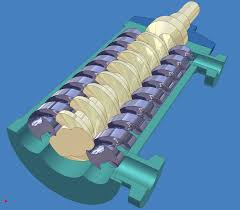
\includegraphics[height=4cm]{figs/simple_screw_pump.jpg}
\hspace{1cm}
\includegraphics[height=5cm]{figs/double-screw_pump.jpg}
\caption{\label{fig:screw_pumps} (left) simple screw pump (right) double-screw pump used for pumping crude oil}
\end{center}
\end{figure}

\noindent Advantages:
\begin{itemize}
\item Practically pulsation-free flow
\item low fluid velocities $\rightarrow$ not sensitive for e.g. sand content
\end{itemize}

\noindent Disadvantages:
\begin{itemize}
\item Expensive
\end{itemize} 

\subsection{Vane pump}

\noindent Advantages:
\begin{itemize}
\item Handles thin liquids at relatively higher pressures
% \item Compensates for wear through vane extension
\item Sometimes preferred for solvents, LPG
\item Can run dry for short periods
% \item Can have one seal or stuffing box
\item Develops good vacuum
\end{itemize}

\noindent Disadvantages:
\begin{itemize}
% \item Can have two stuffing boxes
% \item Complex housing and many parts
\item Not suitable for high pressures
\item Not suitable for high viscosity
\item Not good with abrasives
\end{itemize} 

\noindent Applications:
\begin{itemize}
\item Aerosol and Propellants
\item Aviation Service - Fuel Transfer, Deicing
\item Auto Industry - Fuels, Lubes, Refrigeration Coolants
\item Bulk Transfer of LPG and NH3
\item LPG Cylinder Filling
\item Alcohols
\item Refrigeration - Freons, Ammonia
\end{itemize}

\begin{figure}[ht]
\begin{center}
\includegraphics[height=6cm]{figs/vane_pump.jpg}
\caption{\label{fig:vane_pump} Vane pump}
\end{center}
\end{figure}


\subsection{Progressing cavity pump (eccentric screw pump)}

Widely used for pumping difficult materials such as sewage sludge contaminated with large particles, this pump consists of a helical shaped rotor, about ten times as long as its width. This can be visualized as a central core of diameter x, with typically a curved spiral wound around of thickness half x, although of course in reality it is made from one casting. This shaft fits inside a heavy duty rubber sleeve, of wall thickness typically x also. As the shaft rotates, fluid is gradually forced up the rubber sleeve. Such pumps can develop very high pressure at quite low volumes.

\begin{figure}[h!]
\begin{center}
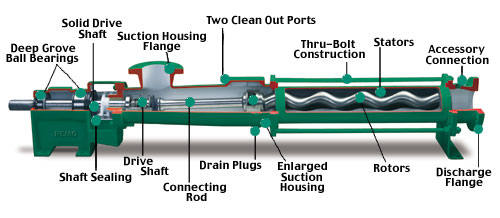
\includegraphics[width=0.7 \textwidth]{figs/cutawaylabel.jpg}
\caption{\label{fig:prog_cav_pumps} Progressive cavity pump.}
\end{center}
\end{figure}


% \frame{\frametitle{Roots-type pumps}
% Named after the Roots brothers who designed and invented it, this lobe pump works by displacing the liquid trapped between two long helical twisted rotors, each fitting into the other when perpendicular at 90°, rotating inside a triangular shaped sealing line configuration, both at the point of suction and at the point of discharge.

% This design produces a continuous flow with equal volume and no vortex. It can work at low pulsation rates and results with gentle performance, more fit for some applications.

% Some applications are:high capacity industrial air compressors, Roots Type Superchargers on internal combustion engines.
% }

\subsection{Peristaltic pump}

A peristaltic pump is a type of positive displacement pump used for pumping a variety of fluids. The fluid is contained within a flexible tube fitted inside a circular pump casing (though linear peristaltic pumps have been made). A rotor with a number of "rollers", "shoes" or "wipers" attached to the external circumference compresses the flexible tube. As the rotor turns, the part of the tube under compression closes (or "occludes") thus forcing the fluid to be pumped to move through the tube. Additionally, as the tube opens to its natural state after the passing of the cam ("restitution") fluid flow is induced to the pump. This process is called peristalsis and is used in many biological systems such as the gastrointestinal tract.

\noindent Advantages

\begin{itemize}
\item No contamination. Because the only part of the pump in contact with the fluid being pumped is the interior of the tube, it is easy to sterilize and clean the inside surfaces of the pump.
\item Low maintenance needs. Their lack of valves, seals and glands makes them comparatively inexpensive to maintain.
\item They are able to handle slurries, viscous, shear-sensitive and aggressive fluids.
\item Pump design prevents backflow and syphoning without valves.[5]
\end{itemize}

\noindent Disadvantages
\begin{itemize}
\item The flexible tubing will tend to degrade with time and require periodic replacement.
\item The flow is pulsed, particularly at low rotational speeds. Therefore, these pumps are less suitable where a smooth consistent flow is required. An alternative type of positive displacement pump should then be considered.
\end{itemize}


\begin{figure}[h!]
\begin{center}
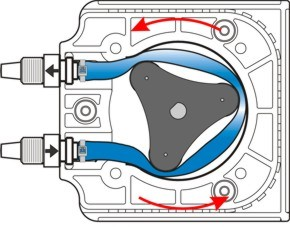
\includegraphics[width=0.4 \textwidth]{figs/per_pumphead.jpg}
\caption{\label{fig:per_pump} Peristaltic pump}
\end{center}
\end{figure}

% \frame{\frametitle{Lobe pump}
% \begin{figure}
% 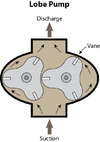
\includegraphics[scale=1]{figs/100px-Common_Lobe_Pump.png}
% \caption{Lobe pump}
% \end{figure}
% }

% \frame{\frametitle{Vane pump}
% }


%%%%%%%%%%%%%%%%%%%%%%%%%%%%%%%%%%%%%%%%%%%%%%%%%%

\clearpage

\subsection{Pulsation dampener}

A pulsation dampener is an accumulator with a set pre-charge that absorbs system shocks while minimizing pulsations, pipe vibration, water hammering and pressure fluctuations. By minimizing pulsation in the system components like regulators, solenoids, sensors, etc., pumps will see decreased wear and have longer life. Pulsation dampeners are tied directly onto the discharge manifold or plumbed immediately downstream of the pump.

\begin{figure}[h]
\begin{center}
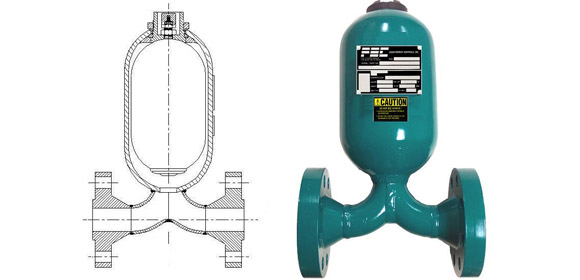
\includegraphics[width=0.8\textwidth]{pulsation_dampeners.jpg}
\caption{\label{fig:pulsation_dampener}Pulsation dampener.}
\end{center}
\end{figure}

The sizing of the dampener goes as follows. The instantaneous and mean flow rate for a single piston pump is 
%
\begin{equation}
Q(t)=Q_{max} \sin (\omega t) \quad \text{and} \quad Q_{mean}=\frac{Q_{max}}{\pi}, \quad \text{where} \quad Q_{max}=\pi A_D s n.
\label{eq:flowratepiston}
\end{equation}
%
The pump flow rate is $Q_p(t)=\sum_{i=1}^N Q_i(t)$, where $Q_i$ is the flow rate of the $i$th piston, i.e. \eqref{eq:flowratepiston} shifted with an angle of $\phi_i=(i-1)\,2\pi/N$, $N$ being the number of pistons. The average flow rate of the pump is $Q_{p,mean}=N\,Q_{mean}$.

The flow rate entering the damper is
%
\begin{equation}
Q_d(t)=Q_p(t)-Q_{p,mean},
\end{equation}
%
while the volume of fluid entering (or leaving) the damper up to time $t$ is
%
\begin{equation}
V_d(t)=\int Q_d(t) dt.
\end{equation}

In the case of a single piston, we have

\begin{align}
Q_d(t)&=\left\{
\begin{matrix}
Q_{max} \left( \sin (\omega t) -\frac{1}{\pi} \right) & \text{if} & 0\leq t \leq \frac{T}{2}\\
-Q_{max}/\pi  & \text{if} & \frac{T}{2}\leq t \leq T
\end{matrix}
\right.
%
\quad 
\text{and}\\
%
V_d(t)&=\left\{
\begin{matrix}
Q_{max} \left( -\frac{1}{\omega}\left(\cos (\omega t)-1\right) -\frac{t}{\pi}\right)  & \text{if} & 0\leq t \leq \frac{T}{2}\\
-t Q_{max} /\pi & \text{if} & \frac{T}{2}\leq t \leq T.
\end{matrix}
\right.
\end{align}

The above expression for $V_d$ also ensures that $V_d(0)=0$. Maximum and minimum volume occurs at $Q_p=0$, i.e.
%
\begin{align}
\omega t_{min}&=\arcsin \frac{1}{\pi} \quad \rightarrow \quad t_{min}=\frac{0.3239}{2 \pi}T=0.0516\,T.\\
\omega t_{max}&=\pi-\arcsin \frac{1}{\pi} \quad \rightarrow \quad t_{max}=\frac{\pi - 0.3239}{2 \pi}T=0.4484\,T.
\end{align}
%
The corresponding volumes are
\begin{equation}
V_{min}=-0.0081\,Q_{max} T=\underbrace{-0.0081 \pi}_{-0.0256} \underbrace{Q_{mean}T}_{V_{stroke}} \quad \text{and} \quad V_{min}=0.1673\,Q_{max} T =0.5256 V_{stroke},
\end{equation}
%
hence the total volume variation on the damper is
%
\begin{equation}
\Delta V=V_{max}-V_{min}=0.55 V_{stroke}
\end{equation}

A similar calculation for a double-acting piston gives
\begin{equation}
t_{min}=0.1098\,T,\quad t_{max}=0.3902\,T\quad \text{and} \quad \Delta V=V_{max}-V_{min}=0.2105 V_{stroke}
\end{equation}

For pumps with 3 or 4 pistons, the analytical derivation is cumbersome, instead, one can simply plot the graphs and evaluate the results numerically giving $\Delta V=0.009 V_{stroke}$ for triplex and $\Delta V=0.044 V_{stroke}$ for four-cylinder pumps, see Figure \ref{fig:pres_damp_volume}. The volume change is given in the percentage of the stroke:
%
\begin{equation}
\shadowbox{$\displaystyle
\Delta V =\nu V_{stroke}, \quad \text{with} \quad 
\left\{ \begin{matrix}
N=&1&2&3&4\\
\nu=&0.55 & 0.21 & 0.044 & 0.009
\end{matrix}
\right.
$}
\end{equation}

\begin{figure}[ht]
\begin{center}
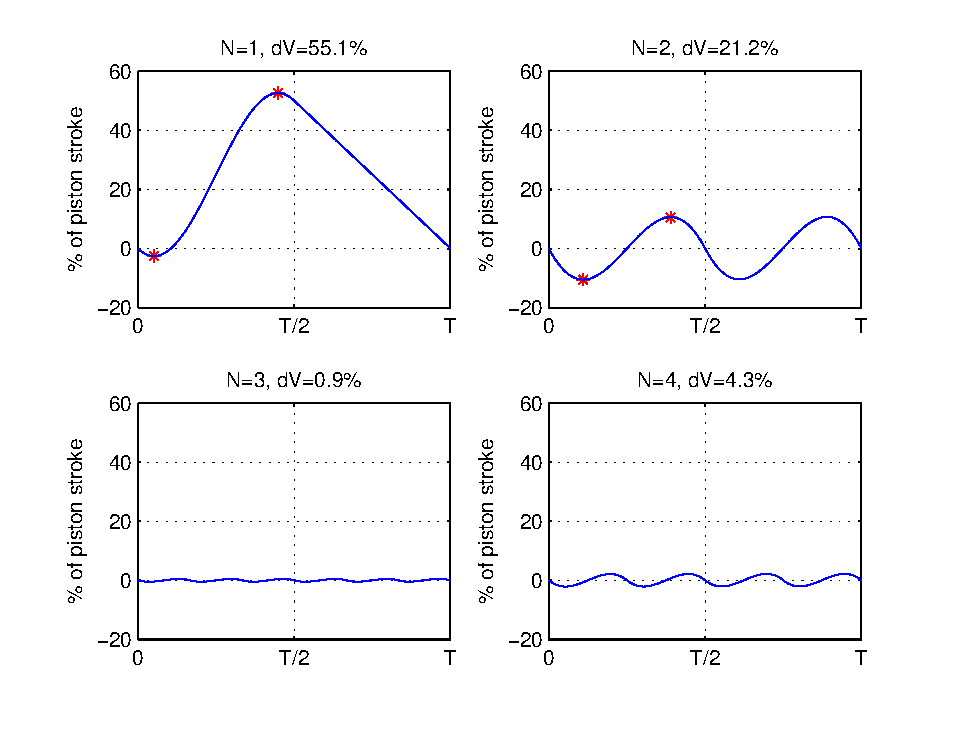
\includegraphics[width=0.8\textwidth]{piston_pumps}
\caption{\label{fig:pres_damp_volume}Volume change in the pressure dampener for different number of pistons.}
\end{center}
\end{figure}

Now let us find the pressure pulsation of the \emph{gas} due to the fluid volume change $\Delta V$. We start off by defining the pre-charge pressure $p_{pc}$ (e.g. 80\% of system pressure), at which the gas volume is $V_0$ (i.e. the nominal volume of the damper) and the required level of damping $\delta=(p_{max}-p_{min})/p_{sys}$. The corresponding \emph{gas} volumes will be $V_{max}$ (corresponding to $p_{min}$) and $V_{min}$ (corresponding to $p_{max}$). At system pressure, the the gas volume is $V_{sys}$. We also have $V^g_{max}=V^g_{min}+\Delta V$.

\noindent Notice that if the process is isotherm (which is usually true in real-life cases), we have)
%
\begin{equation}
\delta =\frac{p_{max}-p_{min}}{p_{sys}} = \frac{\Delta p}{p_{sys}} \approx\frac{\Delta V}{V_{sys}}
\end{equation}
%
\noindent We also have
%
\begin{equation}
p_{min}=p_{pc} \frac{V_0}{V_{max}}, \quad p_{sys}=p_{pc} \frac{V_0}{V_{sys}}\quad \text{and} \quad p_{max}=p_{pc} \frac{V_0}{V_{min}},
\end{equation}
%
and the pressure pulsation level is 
%
\begin{equation}
\delta =\frac{\Delta V}{V_{sys}} = \frac{\nu V_{stroke}}{V_0 \frac{p_{pc}}{p_{sys}}}
\label{eq:delta}
\end{equation}
%
hence the required dampener volume is
%
\begin{equation}
\shadowbox{$\displaystyle
V_0=\frac{\nu V_{stroke}}{\frac{p_{pc}}{p_{sys}} \delta}
$}
\end{equation}


\noindent {\bf Example.} We have a duplex pump ($N=2$, $\nu=0.2105$) with $s=60mm$ stroke and $D=63mm$ diameter.
%
\begin{itemize}
\item The stroke volume is $V_{stroke}=\frac{D^2 \pi}{4}s = 0.187$ liter
\item The precharge pressure is set to 80\% of system pressure: $p_{pc}/p_{sys}=0.8$
\item The required level of damping is $\delta=5\%$.
\item The nominal dampener volume is $V_0=\frac{0.2105 \times 0.187}{0.8\times 0.05}=0.984\approx1$ liter.
\end{itemize}

\clearpage



% PRESSURE RELIEF VALVES %%%%%%%%%%%%%%%%%%%%%%%%%%%%%%%%%%%%%%%%%%%%%%%%%%%%%%
\section{Pressure relief valves (PRVs)} \label{sec:pressure_relief_valve}

It is shown in Sec.\,\ref{sec:basic_characteristics_of_positive_displacement_machines} that the flow rate of a positive displacement pump is hardly affected by the system pressure due to its nearly vertical characteristic curve, see Fig.\,\ref{fig:pump_and_motor_perf_curve}. Therefore, small changes in the flow rate can cause large deviations in the system pressure. In an extreme case, when the volume flow rate of a hydraulic motor needs to be zero (e.g., the motor has to be stopped) and the system is closed by a valve, the pressure will increase almost indefinitely since the pump will provide nearly the same amount volume flow rate regardless of the system pressure. In such cases, the system pressure quickly rises and, if not vented, some component will break, leading to a failure in the equipment. To prevent the excessive increase of the system pressure, a pressure relief valve (PRV) must be mounted {\bf as close to the pump as possible}. These devices open above a pressure threshold value (sometimes called \emph{set pressure} $\Delta p_{set}$) allowing a controlled backflow to the tank or reservoir. If the system pressure is below the set pressure, the PRV remains closed and does not affect the system behaviour. There are two main types of PRVs: direct spring-loaded valves for low flow rate (see Sec.\,\ref{sec:direct_spring_loaded_hydraulic_PRV}), and pilot-operated valves for high flow rate (see Sec.\,\ref{sec:pilot_operated_PRV}).

%------------------------------------------------
\subsection{Direct spring loaded hydraulic PRVs} \label{sec:direct_spring_loaded_hydraulic_PRV}
The first type of pressure relief valve discussed in this section belongs to the family of spring-loaded valves. The main idea is that a valve body or spool is displaced by the system pressure against the force of a pre-compressed spring. If the displacement is large enough, the pressure relief valve opens, and a certain amount of volume flow rate is drained from the system. Direct spring-loaded pressure relief valves are simple and robust, and they can operate with a wide range of chemicals and temperatures. They usually fit into standard piping dimensions. However, they are prone to leakage (if no soft seat is incorporated). In addition, there can be instability issues during their operation called chatter, when the valve body hits the valve seat periodically causing massive damage. The sketch of a piston valve is depicted in Fig.\,\ref{fig:direct_spring_loaded_PRV} and its operation principle is discussed in details in the following.

\begin{figure}[ht!]
	\centering
		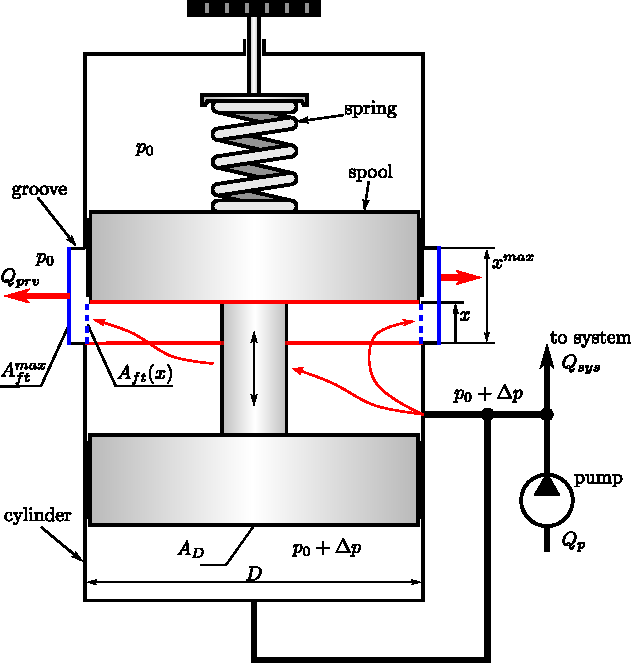
\includegraphics[height=12cm]{PositiveDisplacementPumps/Figures/Direct_Spring_Loaded_PRV.pdf}
	\caption{Scketch of the working principle of a direct spring loaded hydraulic piston pressure relief valve.}
	\label{fig:direct_spring_loaded_PRV}
\end{figure}

The three basic parts of the piston pressure relief valve is a cylinder, a spool (or piston) and a pre-compressed spring. The precompression is usually given as a displacement $x_0$. Depending on the net force acting on the spool, it can move up or down. The force from the spring tries to push the spool downward, which is proportional to the displacement of the spool $x$ (see also the co-ordinate system $x$ in Fig.\,\ref{fig:direct_spring_loaded_PRV}):
%
\begin{equation}
F_s = s (x + x_0),
\end{equation}
%
where $s$ is the spring constant. In contrast, the pressure produced by the pump and guided to the bottom part of the spool pushes the spool upward. The force originated from this system pressure can be written as
%
\begin{equation}
F_p = A_D \Delta p,
\end{equation}
%
where $A_D=D^2 \pi / 4$ is the cross-section of the cylinder or the spool. As usual, $\Delta p$ is the system pressure given as an overpressure. The force balance of the spool reads
%
\begin{equation} \label{force_balance_of_the_spool}
s (x + x_0) = A_D \Delta p.
\end{equation}
%
It is clear that the force of system pressure must overcome the spring force from the precompression $s x_0$ and the spring force increase $s x$ due to the displacement $x$. Thus, the minimum pressure needs to cause any displacement of the spool and start to open the pressure relief valve is
%
\begin{equation} \label{definition_of_set_pressure}
\Delta p_{set} = \frac{s x_0}{A_D},
\end{equation}
%
where $\Delta p_{set}$ is called the opening pressure or the \textit{set pressure}. The value of $\Delta p_{set}$ clearly separates the closed and opened states of the pressure relief valve. If $\Delta p < \Delta p_{set}$, the valve is closed; that is, the edge of the spool marked by the red line in Fig.\,\ref{fig:direct_spring_loaded_PRV} is below the other red horizontal line associated to the cylinder that represents the zero displacement of the spool (x=0). In contrast, when $\Delta p > \Delta p_{set}$, the relative position of the two red lines is the opposite, and the valve is opened. This means that hydraulic fluid (usually oil) flows through the groove formed somewhere in the middle of the cylinder. The flow direction is marked by the red arrows in Fig.\,\ref{fig:direct_spring_loaded_PRV}. The \textit{cylindrical} outflow area is depicted by the vertical dashed blue lines and labelled by $A_{ft}(x)$. The dependence on the displacement $x$ emphasizes that the cross-flow area depends on the system pressure $\Delta p$, see also Eq.\,\eqref{force_balance_of_the_spool}. Thus, the volume flow rate $Q_{prv}$ through the pressure relief valve increases with $\Delta p$ not only by the larger pressure difference but because of the increasing cross-section as well. The cross-section $A_{ft}$ increases up to a limit point with $x$. If the displacement reaches $x^{max}$, the red edge of the spool moves beyond the upper limit of the groove, and the cross-section is fixed at $A_{ft}^{max}$ (solid blue lines in Fig.\,\ref{fig:direct_spring_loaded_PRV}). In this situation, the volume flow rate of the pressure relief valve $Q_{prv}$ can be increased only by the increase of the pressure difference $\Delta p$. In summary, three different stages can be defined to determine the general mathematical form of the cross-section $A_{ft}(x)$:
%
\begin{equation} \label{flow_cross_section_of_pressure_relief_valve}
A_{ft}(x) =
	\begin{cases}
		0 & \mathrm{for} \quad x<0, \\
		D \pi x = D \pi \left( \dfrac{A_D\Delta p}{s} - x_0 \right) & \mathrm{for} \quad 0<x<x^{max}, \\
		D \pi x^{max} & \mathrm{for} \quad x>x^{max}.
	\end{cases}
\end{equation}
%
Obsere that for the case $0<x<x^{max}$, Eq.\,\eqref{force_balance_of_the_spool} is employed.

The main task now is to determine the characteristic curve of the pressure relief valve, which is the relationship of the volume flow rate $Q_{prv}$ and the pressure difference $\Delta p$. From the Bernoulli equation, assuming ideal fluid flow (without losses), the theoretical velocity through a cross-section $A$ having a pressure difference $\Delta p$ between its two sides is
%
\begin{equation}
v_{th} = \sqrt{ \frac{2 \Delta p}{\rho} },
\end{equation}
%
where $\rho$ is the density of the working fluid. The theoretical volume flow rate is simply
%
\begin{equation}
Q_{th} = A v_{th} = A \sqrt{ \frac{2 \Delta p}{\rho} }.
\end{equation}
%
In reality, the fluid flow is far from ideal; thus, the equation for the flow rate can be written as
%
\begin{equation}
Q_{th} = C_d A \sqrt{ \frac{2 \Delta p}{\rho} },
\end{equation}
%
where $C_d$ a flow factor usually determined empirically. So far, $v_{th}$, $Q_{th}$ and $A$ are general notations of the velocity, volume flow rate and cross-section, respectively. Specifically, in case of the pressure relief valve, the general function of the volume flow rate $Q_{prv}(\Delta p)$ can be written as
%
\begin{equation}
Q_{prv}(\Delta p) = C_d A_{ft}(x) \sqrt{ \frac{2 \Delta p}{\rho} },
\end{equation}
%
which is a piecewise smooth function according to the formulae in equation Eq.\,\eqref{flow_cross_section_of_pressure_relief_valve} for the corss-section $A_{ft}(x)$:
%
\begin{equation} \label{general_volume_flow_rate_PRV}
Q_{prv}(\Delta p) =
	\begin{cases}
		0 & \mathrm{for} \quad x<0, \\
		C_d D \pi  \left( \dfrac{A_D \Delta p}{s} - x_0 \right) \sqrt{ \dfrac{2 \Delta p}{\rho} } & \mathrm{for} \quad 0<x<x^{max}, \\
		C_d D \pi x^{max} \sqrt{ \dfrac{2 \Delta p}{\rho} } & \mathrm{for} \quad x>x^{max}.
	\end{cases}
\end{equation}
%
Note that in the middle range, we have
%
\begin{equation} \label{volume_flow_rate_middle_range_PRV}
Q_{prv}(\Delta p) = C_d D \pi\frac{A_D}{s} \left( \Delta p - \frac{s x_0}{A_D} \right) \sqrt{ \frac{2 \Delta p}{\rho} } = C_1 \left( \Delta p - \Delta p_{set} \right) \sqrt{\Delta p} = C_1 \left( \Delta p^{3/2} - \Delta p_{set} \Delta p^{1/2} \right),
\end{equation}
%
where the factor $C_1$ accumulates all the constants presented in the equation. Equation\,\eqref{volume_flow_rate_middle_range_PRV} has two roots: $\Delta p=0$ and $\Delta p = \Delta p_{set}$ (comparing Eqs.\,\eqref{force_balance_of_the_spool} and \eqref{definition_of_set_pressure}, in this case $x=0$). When $\Delta p > \Delta p_{set}$, the dominating term is $\Delta p^{3/2}$. Similarly, the last range in Eq.\,\eqref{general_volume_flow_rate_PRV} is
%
\begin{equation}
Q_{prv}(\Delta p) = C_2 \sqrt{\Delta p} = C_2 \Delta p^{1/2},
\end{equation}
%
which has a single root at $\Delta p=0$, and $C_2$ again accumulates all the constants in the equation.

The left panel of Fig.\,\ref{fig:characteristic_curve_of_PRV} shows the ``assembling'' of the effective characteristic curve ($Q_{prv}-\Delta p$ diagram) of a pressure relief valve, which is composed by segments obtained from the general expression of Eq.\eqref{general_volume_flow_rate_PRV}. If the system pressure $\Delta p<\Delta p_{set}$, the pressure relief valve is closed, and the volume flow rate is zero $Q_{prv}=0$, see the red horizontal line in the left-hand side of Fig.\,\ref{fig:characteristic_curve_of_PRV}. Keep in mind again that the limit case $\Delta p=\Delta p_{set}$ corresponds to the zero displacement $x=0$ (the coincidence of the two red horizontal lines in Fig.\,\ref{fig:direct_spring_loaded_PRV}). When the system pressure is greater than the set pressure ($\Delta p>\Delta p_{set}$), the pressure relief valve is open, and the released volume flow rate explicitly depends on the system pressure $\Delta p$ and implicitly on the displacement $x$. The two functions of the last two ranges in Eq.\,\eqref{general_volume_flow_rate_PRV} is represented by the black solid curves in the left-hand side of Fig.\,\ref{fig:characteristic_curve_of_PRV}; their equations are also highlighted in the diagram. Although the boundary between the validity limit of the two functions is known to be $x^{max}$, it is not known explicitly in terms of the system pressure $\Delta p$; however, it appears as a crossing of the two black curves. Between the points of $\Delta p_{set}$ and the crossing, the middle function in Eq.\,\eqref{general_volume_flow_rate_PRV} is valid (range $0<x<x^{max}$). The corresponding segment is highlighted by red. Above the crossing (maximum displacement $x^{max}$), the pressure relief valve operates along the function presented by the last expression in Eq.\,\eqref{general_volume_flow_rate_PRV}. This part of the curve is coloured by red as well. In summary, the effective characteristic curve of a pressure relief valve is composed of three segments connected continuously (but not smoothly) depending on the displacement $x$ of the spool.

\begin{figure}[ht!]
	\centering
		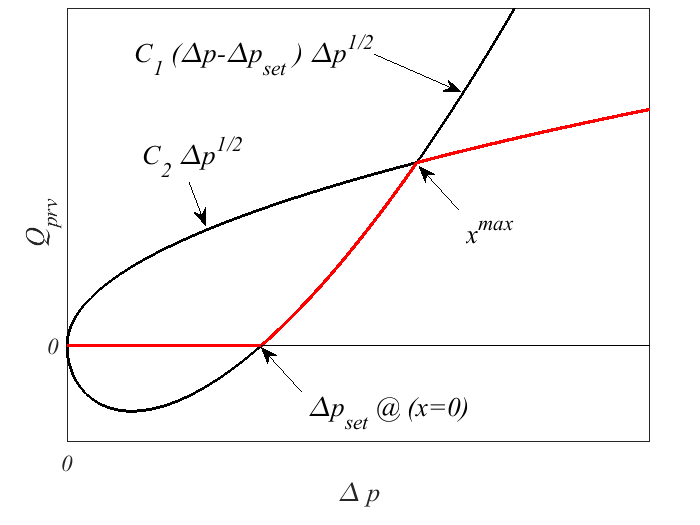
\includegraphics[width=8cm]{PositiveDisplacementPumps/Figures/Characteristic_Curves_Of_Pressure_Relief_Valves_Dp_Q.png}
		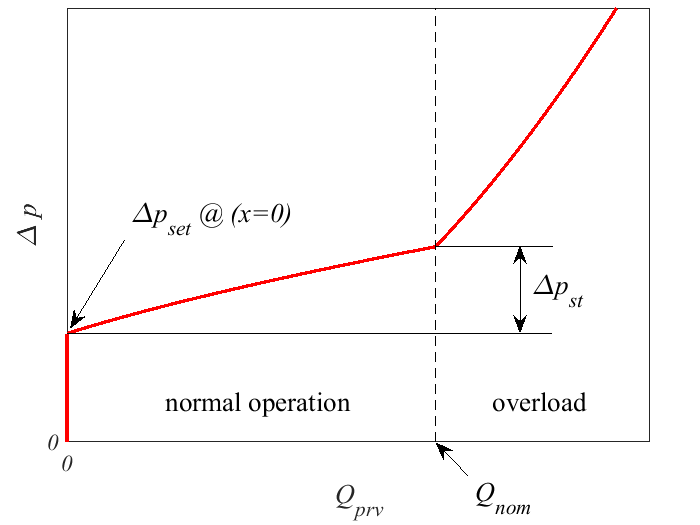
\includegraphics[width=8cm]{PositiveDisplacementPumps/Figures/Characteristic_Curves_Of_Pressure_Relief_Valves_Q_Dp.png}
	\caption{A typical characteristic curve of a spring-loaded pressure relief valve. Left: the volume flow rate $Q_{prv}$ as a function of the pressure difference $\Delta p$. The theoretical (black) curves are also depicted. Right: the pressure difference $\Delta p$ as a function of the flow rate $Q_{prv}$.}
	\label{fig:characteristic_curve_of_PRV}
\end{figure}

The usual way of plotting the characteristic curve (also in the catalogue) is the inverse of the $Q_{prv}(\Delta p)$ function. It is shown in the right-hand side of Fig.\,\ref{fig:characteristic_curve_of_PRV}. The volume flow rate at the maximum displacement $x^{max}$ (at the break of the characteristic curve) is called the nominal flow rate $Q_{nom}$. This is the maximum possible flow rate the pressure relief valve can drain away without reaching the maximum displacement $x^{max}$. The range between $Q_{prv}=0$ and $Q_{prv}=Q_{nom}$ is called normal operation; whereas, the operation with $Q_{prv}>Q_{nom}$ is called overload. The optimal case in the normal operation would be the absolute horizontal line of the characteristic curve. That is, in case of opening, the pressure relief valve prevents the increase the system pressure above $\Delta p_{set}$. However, this condition cannot be satisfied as the increasing flow rate need bigger pressure difference as a driving force. The reason for the slight increase is due to the increasing cross-section of the fluid flow. Thus, there will always be a small overshoot above $\Delta p_{set}$. The largest of such an overshoot in the normal operation range (at $x^{max}$) is called static error $\Delta p_{st}$ depicted also in the right-hand side of Fig.\,\ref{fig:characteristic_curve_of_PRV}. Note that Fig.\,\ref{fig:characteristic_curve_of_PRV} do not present a real characteristic curve, it serves only demonstration purposes. In reality, the static error very small, it is about $\Delta p_{st} \approx (0.01 \dots 0.1) \Delta p_{set}$.

\begin{figure}[ht!]
	\centering
		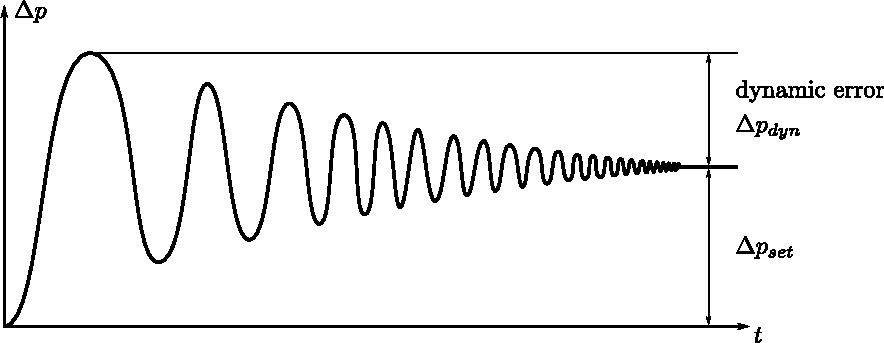
\includegraphics[width=12cm]{PositiveDisplacementPumps/Figures/Dynamic_Error_Pressure_Relief_Valve.pdf}
	\caption{Dynamic error of a direct spring-loaded hydraulic pressure relief valve (PRV) in case of a quick opening.}
	\label{fig:dynamic_error_of_direct_spring_loaded_PRV}
\end{figure}

Large error (deviation from the $\Delta p_{set}$) can occur during the transient dynamics of the valve body or spool of a pressure relief valve. In case of a sudden increase of the system pressure $\Delta p$ above the threshold value $\Delta p_{set}$, the pressure relief valve has to open quickly and release as much flow rate as possible to normalize or prevent the further increase of the system pressure $\Delta p$. However, the opening cannot happen infinitely fast (that would need infinitely large force); consequently, the valve body or the spool has its own dynamics governed by its mass, the spring characteristics and the system pressure. In reality, when the valve body is accelerated to a certain velocity, it cannot be stoped at the required position (due to its inertia) and the opening (displacement) increases further. This will cause a decrease in the system pressure as the displacement and the cross-section of the outflow is bigger than necessary (in steady-state operation). Due to the drop in the system pressure, the pressure relief valve starts to close, and an overshoot in the displacement happens again but in the opposite (negative) direction. The result is a temporary increase in the system pressure, and the cycle repeats again. Hopefully, these oscillations decay in time, e.g., due to the viscous forces of the hydraulic fluid. The discussion of the exact dynamics and the governing equations are beyond the scope of this subject; however, it is important to keep in mind the phenomenon. For demonstration purposes, a typical system pressure evolution in time is depicted in Fig.\,\ref{fig:dynamic_error_of_direct_spring_loaded_PRV} of a quick opening. The maximum overshoot in the system pressure is called dynamic error $\Delta p_{dyn}$ that can be much higher than the static error $\Delta p_{st}$ (even $2$ or $3$ times larger). It is worth noting that for certain configurations, the amplitude of the oscillations can increase. Naturally, the oscillation amplitude has a definite physical constrain when the valve body or the spool hits the valve seat or the wall of the cylinder. Such an operating condition can cause massive damage in the pressure relief valve. This scientific area is still actively researched (also by our department supervised by Csaba H\H{o}s) as there is no trivial answer for under what conditions such instabilities arise.

\begin{figure}[ht!]
	\centering
		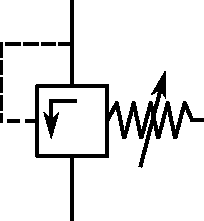
\includegraphics[width=3cm]{PositiveDisplacementPumps/Figures/Standard_Symbol_Of_Pressure_Relief_Valves.pdf}
	\caption{Standard symbol of pressure relief valves in block diagrams of hydraulic systems.}
	\label{fig:standard_symbol_of_PRV}
\end{figure}

The standard symbol of a direct spring-loaded pressure relief valve used in block diagrams of hydraulic systems is depicted in Fig.\,\ref{fig:standard_symbol_of_PRV}. The arrow at the spring symbol means adjustable pre-compression. The dashed line indicates that the valve opens by the system pressure against the spring force (opposite side). Hypothetically, in case of opening, the arrow inside the solid square is aligned with the piping (vertical lines at the top and the bottom of the square).

Finally, let us discuss how the proper size of a pressure relief valve can be selected. First of all, it is customary to choose the set (opening) pressure above approximately $20\%$ of the designed system pressure; namely, $\Delta p_{set} \approx 1.2 \Delta p$. For the details of the proper determination of the system pressure $\Delta p$, see Sec.\,\ref{sec:sizing_of_hydraulic_systems}. Naturally, the construction of the valve has to withstand this pressure. Another factor during the selection is the nominal flow rate $Q_{nom}$. In case of a sudden emergency closure of the system, the pressure relief valve needs to be able to release all the flow rate back to the reservoir produced by the pump. Moreover, it must be done in the normal operation conditions already explained in the right-hand side of Fig.\,\ref{fig:dynamic_error_of_direct_spring_loaded_PRV}. Mathematically, this means that
%
\begin{equation}
Q_{nom} > Q_{p}^{max}.
\end{equation}

%------------------------------------------------
\subsection{Hydraulic aggregate}
As already explained in the introduction of Sec.\,\ref{sec:pressure_relief_valve}, due to safety reasons, a hydraulic pump is never used alone to provide power to a hydraulic system. It is always combined with a pressure relief valve (PRV) to release a certain amount of flow rate back to the reservoir if the system pressure exceeds a threshold value. Actually, the pump and a built-in pressure relief valve are inherently used together. Thus, during the design and/or control process of a hydraulic system, the combined characteristic curve of a pump-PRV unit is taken into consideration. The pump and the pressure relief valve are connected in parallel illustrated by the block diagram in Fig.\,\ref{fig:hydraulic_aggregate}.

\begin{figure}[ht!]
	\centering
		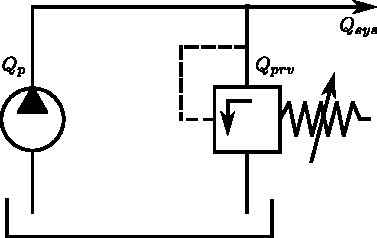
\includegraphics[height=3.5cm]{PositiveDisplacementPumps/Figures/Block_Diagram_Hydraulic_Aggregate.pdf}
	\caption{Block diagram of a hydraulic aggregate composed by a pump and a pressure relief valve connected in parallel.}
	\label{fig:hydraulic_aggregate}
\end{figure}

If the system pressure exceeds the opening pressure ($\Delta p > \Delta p_{set}$), the pressure relief valve opens and $Q_{prv}$ amount of flow rate is released back immediately to the reservoir. Therefore, the flow rate observed by the system $Q_{sys}$ is less than the one produced by the pump:
%
\begin{equation} \label{system_flow_rate_hydraulic_aggregate}
Q_{sys} = Q_p - Q_{prv}.
\end{equation}
%
The characteristic curve of the hydraulic aggregate is the system pressure $\Delta p$ as a function of the system flow rate $Q_{sys}$. The main aim of this section is to compose this characteristic curve from the already known characteristic curves of the pump and the pressure relief valve.

\begin{figure}[ht!]
	\centering
		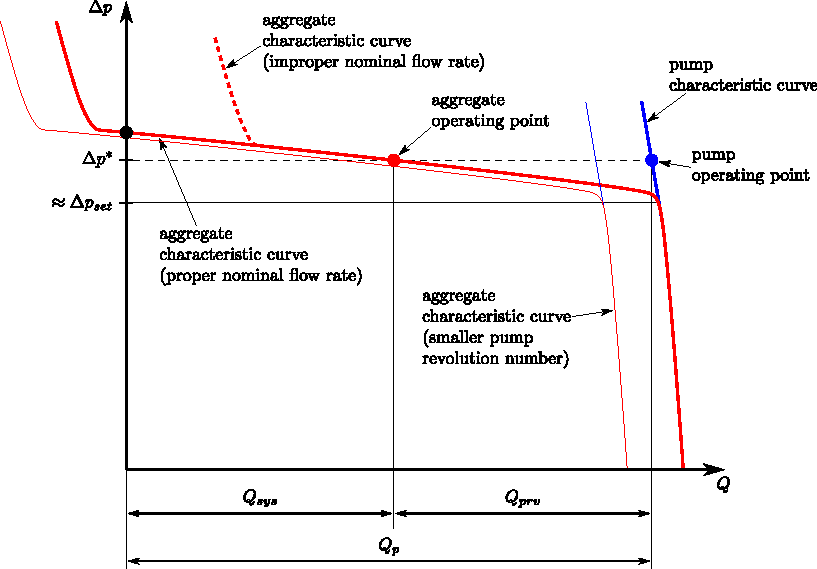
\includegraphics[height=9.75cm]{PositiveDisplacementPumps/Figures/Characteristic_Curve_Hydraulic_Aggregate.pdf}
	\caption{Typical characteristic curves of a hydraulic aggregate with proper nominal flow rate (solid red curve) and improper nominal flow rate (dashed red curve). The characteristic curve of the pump is denoted by the blue curve (partially overlapped with the solid red curve). The thin red and blue lines represent characteristic curves with a lower pump revolution number or with a different pump having lower output flow rate (the pressure relief valve is the same).}
	\label{fig:characteristic_curve_hydraulic_aggregate}
\end{figure}

The ``shape'' of the characteristic curve of a hydraulic aggregate can be estimated with good confidence by inspecting Eq.\,\eqref{system_flow_rate_hydraulic_aggregate}. If we assume that the pump volume flow rate is nearly constant (nearly independent from the system pressure $\Delta p$), which is fairly valid, the characteristic curve of the hydraulic aggregate can be obtained simply by mirroring the characteristic curve of the pressure relief valve to the vertical axis (due to the negative sign in front of $Q_{prv}$), and shift it by the nearly constant $Q_p$ towards the positive direction of the volume flow rate.

Such a characteristic curve is presented in Fig.\,\ref{fig:characteristic_curve_hydraulic_aggregate} by the solid thick red curve. The characteristic curve of the pump is the solid blue line that coincides with the red curve below the set (opening) pressure $\Delta p_{set}$ (the pressure relief valve is closed, $Q_{prv}=0$ and $Q_{sys}=Q_p$), see also the horizontal thin black line. Observe that the characteristic curve here is slightly inclined because of the volumetric efficiency of the pump. When the system pressure $\Delta p$ increases above the set pressure, the pressure relief valve opens, and the system volume flow rate starts to decrease according to Eq.\,\eqref{system_flow_rate_hydraulic_aggregate}. Thus, the red and blue solid curves separate. The red curve has only a slightly inclined plateau (according to the discussion in Sec.\,\ref{sec:direct_spring_loaded_hydraulic_PRV}) meaning that a small increment in the system pressure results in a significant increment of $Q_{prv}$ and large decrement of $Q_{sys}$. In a limit case, if the system pressure is high enough, the system flow rate is $Q_{sys}=0$, and $Q_p=Q_{prv}$. This happens where the solid red curve crosses the vertical axis denoted by the black dot. Here, all the flow rate produced by the pump flows back to the reservoir immediately through the pressure relief valve.

An example for the distribution of the flow rates at a system pressure of $\Delta p=\Delta p^*$ is also shown in Fig.\,\ref{fig:characteristic_curve_hydraulic_aggregate}. The crossings of the dashed horizontal line with the red and the solid blue curves define the operation points of the hydraulic aggregate (red dot) and the pump (blue dot), respectively. The magnitudes of the corresponding flow rates $Q_{sys}$, $Q_{prv}$ and $Q_p$ are highlighted by the arrows in the bottom of the figure.

The characteristic curve of the hydraulic aggregate continues further in the negative regions of the system flow rate. Although such operation has no practical relevance (the flow rate $Q_{prv}$ is fed both from the pump and the system side), it is crucial that third part of the characteristic curve, where the system pressure starts to increase rapidly (compare also with Fig.\,\ref{fig:characteristic_curve_of_PRV}), should be in this domain. That is, the nominal flow rate $Q_{nom}$ have to be large enough to be able to release the maximum possible flow rate of the pump back to the reservoir. If the pressure relief valve is poorly selected, and the nominal flow rate is too small, the characteristic curve of the hydraulic aggregate looks like the red dashed curve in Fig.\,\ref{fig:characteristic_curve_hydraulic_aggregate}. In this case, if a total closure happens, the pressure relief valve cannot keep the system pressure near the set pressure $\Delta p_{set}$, which can lead to failure.

As a final remark, if the revolution number of the pump decreases (increases), the characteristic curve of the hydraulic aggregate is shifted towards the negative (positive) direction of the flow rate. Similar transformation happens if the pump is replaced by another one having a smaller (larger) flow rate (e.g., due to the smaller geometric volume). Such an example is depicted by the thin red and blue curves in Fig.\,\ref{fig:characteristic_curve_of_PRV}. The main reason is the shift of the characteristic curve of the pump with changing revolution number, see again Fig.\,\ref{fig:pump_and_motor_perf_curve} and the discussion in Sec.\,\ref{sec:basic_characteristics_of_positive_displacement_machines}.

%------------------------------------------------
\subsection{Pilot operated hydraulic PRVs} \label{sec:pilot_operated_PRV}
One of the main disadvantages of direct spring-loaded pressure relief valves is when the (nominal) volume flow rate increases, the static error $\Delta p_{st}$ can increase to an unacceptable level. This behaviour can be clearly seen in the right-hand side of Fig.\,\ref{fig:characteristic_curve_of_PRV} in the increasing nature of the characteristic curve of the valve in the normal operating regime. The main reason is that the displacement $x$ (``amount'' of opening) depends on the system pressure itself, see the middle range in Eq.\,\eqref{general_volume_flow_rate_PRV} repeated here:
%
\begin{equation}
Q_{prv} = C_d D \pi  \underbrace{ \left( \dfrac{A_D \Delta p}{s} - x_0 \right) }_{x} \sqrt{ \dfrac{2 \Delta p}{\rho} } = 
 C_d D \pi \frac{A_D}{s} \bigg( \Delta p - \underbrace{\frac{s x_0}{A_D}}_{\Delta p_{set}} \bigg) \sqrt{ \dfrac{2 \Delta p}{\rho} }.
\end{equation}
%
That is, in order to increase the volume flow rate $Q_{prv}$, it is inevitable to increase the system pressure $\Delta p$ (thus the static error $\Delta p_{st}$) as well. The technical difficulty is how to increase the flow rate $Q_{prv}$ for the same level of $\Delta p$ without altering the set pressure $\Delta p_{set}$. A natural option is to increase the diameter of the cylinder $D$ that will increase the cross-section of the outflow in general, which will decrease the static error of the pressure relief valve. However, as the set pressure
%
\begin{equation} \label{set_presusre_adjustment}
\Delta p_{set} = \frac{s x_0}{A_D} = \frac{4 s x_0}{D^2 \pi}
\end{equation}
%
depends also on the diameter $D$, it must be corrected either by the spring constant $s$ or the pre-compression $x_0$.

Let us investigate the dependence of the static error $\Delta p_{st}$ on the variation of the diameter of the cylinder $D$. From the right-hand side of Fig.\,\ref{fig:characteristic_curve_of_PRV}, one can conclude that the bigger the solpe
%
\begin{equation}
\frac{d Q_{prv}}{d \Delta p} = \frac{d}{d \Delta p} \left( C_d D \pi \frac{D^2 \pi}{4 s} \sqrt{\frac{2}{\rho}} \Delta p^{3/2}\right) \propto \frac{D^3}{s} \sqrt{\Delta p}
\end{equation}
%
of the characteristic curve in the normal operation, the larger the resulted static error $\Delta p_{st}$. That is, we can write:
%
\begin{equation} \label{static_error_dependency}
\Delta p_{st} \propto \frac{d Q_{prv}}{d \Delta p} \propto \frac{D^3}{s}
\end{equation}
%
when the system pressure $\Delta p$ is kept at the same level. Adjusting the set pressure via the spring constant, which is proportional to the second power of the diameter ($s \propto D^2$) according to Eq.\,\eqref{set_presusre_adjustment}, the static error is proportional to the first power of the diameter $D$:
%
\begin{equation}
\Delta p_{st} \propto \frac{d Q_{prv}}{d \Delta p} \propto \frac{D^3}{s} \propto D.
\end{equation}
%
In contrast, adjusting the set pressure via the pre-compression $x_0$, the static error is proportional to the third order of the diameter $D$:
%
\begin{equation}
\Delta p_{st} \propto \frac{d Q_{prv}}{d \Delta p} \propto \frac{D^3}{s} \propto D^3,
\end{equation}
%
since the precompression $x_0 \propto D^2$, see again Eq.\,\eqref{set_presusre_adjustment}, does not appear in Eq\,\eqref{static_error_dependency}.

In summary, the magnitude of the static error can be decreased by increasing the diameter of the cylinder $D$, which increases the cross-section of the outflow. In this case, the set pressure must be adjusted via the spring constant $s$ or the pre-compression $x_0$. In both cases, adjustment by $s$ or $x_0$, the static error is proportional to the first and third power of $D$, respectively. That is, the magnitude of the static error can only be softened, but cannot be eliminated by varying $D$. Moreover, the adjustment by $s$ is more effective compared to the adjustment by $x_0$.

An efficient solution for the above-described problem is the usage of a pilot operated pressure relief valve. The sketch of a pilot operated valve is shown in Fig.\,\ref{fig:direct_spring_loaded_PRV}. Its operation principle is discussed in details in the rest of this section. The main part of the construct is the cylinder, the spool positioned by a soft spring (low value of the spring constant), and the pilot having a hard spring (large spring constant) and opened via an orifice. First of all, let us assume that the pilot is closed. In this case, the pressure is the same in the upper, middle, and the lower part of the spool since all these three chambers are connected to the same system pressure. Thus, the net force acting on the spool is determined by the soft spring alone. Even if the spring is very soft, it can ensure the closure of the pressure relief valve by the spool.

The critical setup of the device is the spring constant of the hard spring and its pre-compression. These quantities determine the set pressure $\Delta p_{set}$ of the pressure relief valve. That is, the pressure relief valve opens when the pilot opens. Now imagine that the pilot is opened due to the increasing system pressure $\Delta p$. In this case, the pressure is dropped in the chamber above the spool (the pressure is ``relieved'' from this chamber). Due to the fixed orifice (acts as a resistance) in the pipe connected to this chamber, the pressure cannot recover fast by the pump. Therefore, there is an imbalance between the upper and lower part of the spool resulted in its large displacement. Keep in mind that the soft spring connected to the spool can compensate only a small pressure difference. In this way, large displacement (significant flow rate $Q_{prv}$) can be achieved even if the system pressure $\Delta p$ is only slightly above the set pressure $\Delta p_{set}$. This feature makes the pilot-operated pressure relief valves a viable option if the static error must definitely be kept within a low level.

\begin{figure}[ht!]
	\centering
		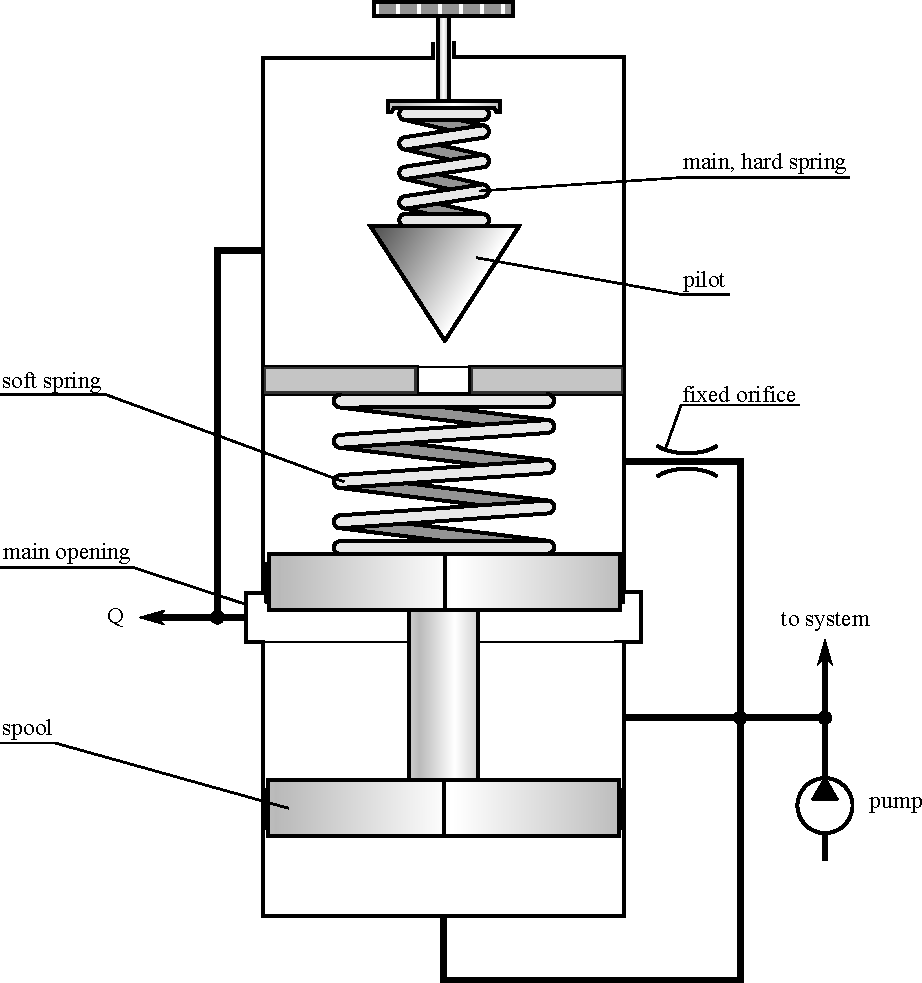
\includegraphics[height=12cm]{PositiveDisplacementPumps/Figures/Pilot_Operated_PRV.pdf}
	\caption{Scketch of the working principle of a pilot operated pressure relief valve.}
	\label{fig:pilot_operated_PRV}
\end{figure}

% SIZING EXAMPLES OF SIMPLE HYDRAULIC SYSTEMS %%%%%%%%%%%%%%%%%%%%%%%%%%%%%%%%%
\section{Sizing examples of simple hydraulic systems} \label{sec:sizing_of_hydraulic_systems}

In the previous sections, the basic components (e.g., pumps, motors, pressure relief valve and hydraulic aggregate) of hydraulic systems and their characteristic curves are discussed in details. In the present section, the already acquired knowledge is put together, and the fundamentals of complex hydraulic systems are examined. Essentially, all-hydraulic circuits are the same regardless of the application. There are six basic components required for setting up a hydraulic system, which are as follows. Reservoir(s) to hold the liquid (usually hydraulic oil). Pump(s) to force the liquid through the system. Electric motor(s) or other power source(s) (e.g., diesel engine) to drive the pump(s). Valves to control the liquid direction, pressure and flow rate. Actuator(s) to convert the energy of the liquid into mechanical force or torque, to do useful work. Actuators can either be cylinders that provide linear motion or motors that provide rotary motion. Finally, piping to convey the liquid from one location to another is also necessary. Figure\,\ref{Fig:Examples_of_hydraulic_systems} shows a simple (left) and a more complex (right) examples of real hydraulic applications (this figure serves as demonstration purposes of the possible complexities, and the details are not important here).

\begin{figure}[ht!]
	\centering
		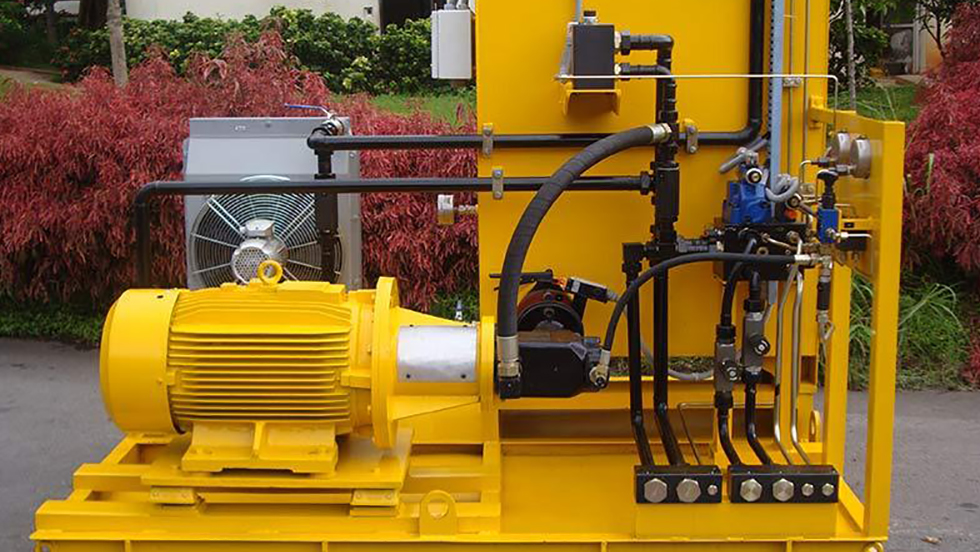
\includegraphics[height=4.5cm]{PositiveDisplacementPumps/Figures/Example_Of_Hydraulic_System_1.jpg}
		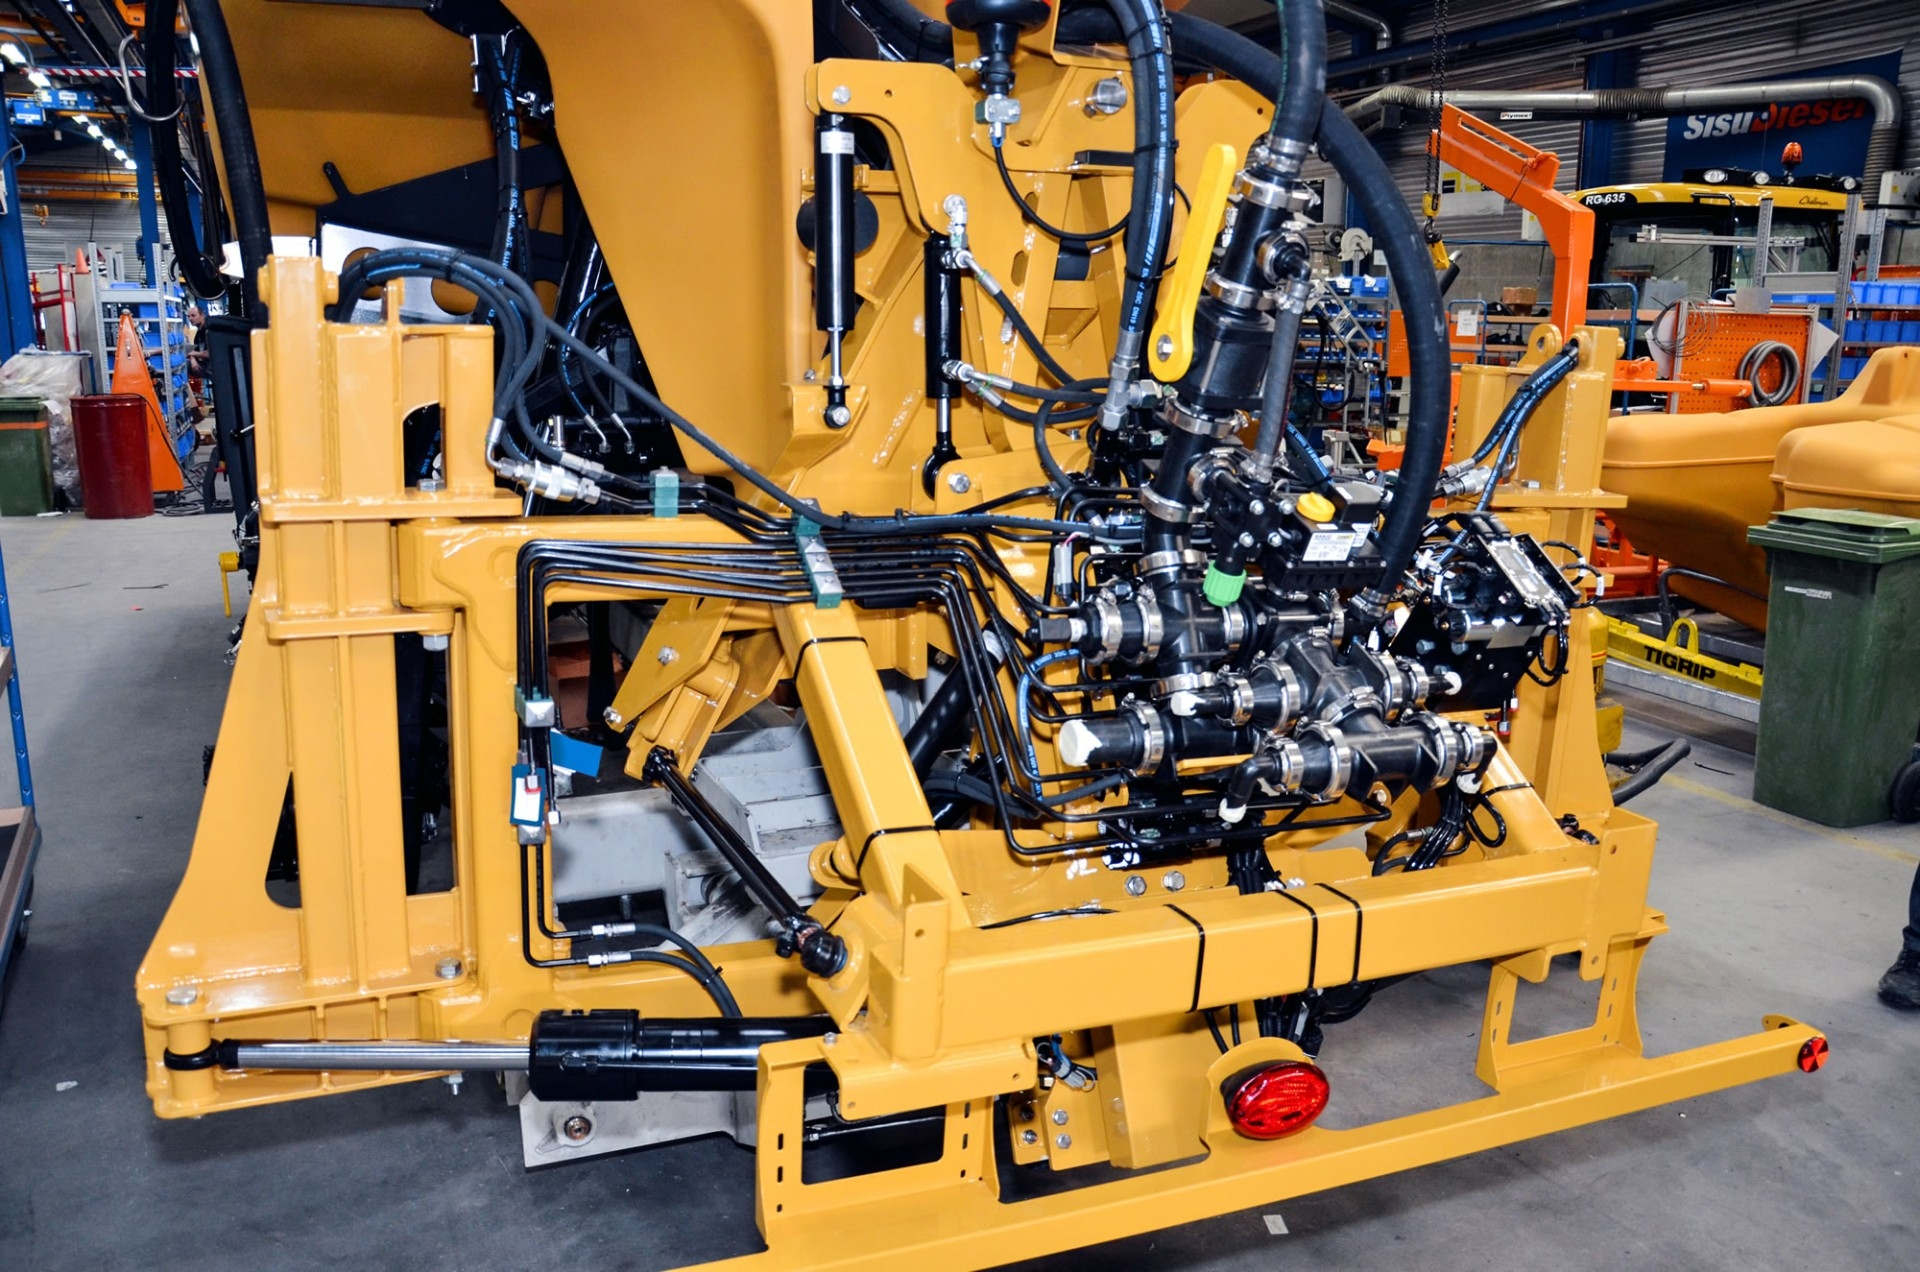
\includegraphics[height=4.5cm]{PositiveDisplacementPumps/Figures/Example_Of_Hydraulic_System_2.jpg}
	\caption{Two typical examples of real hydraulic applications.}
	\label{Fig:Examples_of_hydraulic_systems}
\end{figure}

Using hydraulic systems have many advantages that make them suitable in a large variety of applications. For example, hydraulic systems can be used in environments involving dirt and underwater. A hydraulic motor can be stopped under heavy load without damage (in contrast, e.g., to electric motors). High torque can be generated with small size, which is independent of the flow rate (velocity or angular velocity). Last but not least, such a solution allows a fast change of velocity or revolution number or even the direction of the linear motion or rotation.

Due to the precise and fast response, hydraulic systems are widely used in many industrial projects: plastic processing machinery, steel making and primary metal extraction applications, automated production lines or machine tool industry, to name a few. In mobile hydraulics, it is used in building and construction equipment like cranes, excavators, backhoe or earth moving equipment. The most important applications in the automobile industry are the power steering and brake systems. Hydraulics plays a vital role in marine applications, e.g., to maintain the stability and control of ships. As a final example, hydraulic fracturing is one of the advanced mining technology used for extracting unused gases/oils beneath the earth surface.

In the following sections, the basic process of the sizing of simple hydraulic systems is introduced. That is, how the hydraulic components for a given task (linear or rotary motion) can be chosen, and how the operation of the system can be controlled/ragulated.

%------------------------------------------------
\subsection{A hydraulic system with hydraulic motor} \label{sec:hydraulic_system_with_hydraulic_motor}
Let us consider a hydraulic system where a hydraulic aggregate drives a hydraulic motor. A hydraulic motor is a mechanical actuator that converts hydraulic pressure and flow rate into torque and angular displacement (rotation). Conceptually, a hydraulic motor should be interchangeable with a hydraulic pump because it performs the opposite function - similar to the way a DC electric motor is theoretically interchangeable with a DC electrical generator. However, many hydraulic pumps cannot be used as hydraulic motors because they cannot be back driven. Also, a hydraulic motor is usually designed for working pressure at both sides of the motor, whereas most hydraulic pumps rely on low pressure provided from the reservoir at the input side and would leak fluid when abused as a motor.

The block diagram of the simplest such a hydraulic system is presented in Fig.\,\ref{fig:hydraulic_aggregate_with_motor}. The heart of the system is the hydraulic aggregate composed by a pump and a pressure relief valve, see also Sec.\,\ref{sec:pressure_relief_valve} for details, which provides the volume flow rate $Q$ and the pressure difference $\Delta p$ to the system. The opening pressure of the pressure relief valve $\Delta p_{set}$ should be higher than the operating pressure difference of the system $\Delta p$. The pump is usually driven by an electric motor or a diesel engine with torque $M_e=M_p$ and revolution number $n_e=n_p$. Here the subscripts $e$ and $p$ means electric motor and pump, respectively. The pump has a geometric volume $V_{g,p}$. The hydraulic power is transferred to the hydraulic motor through the piping depicted by the black lines in Fig.\,\ref{fig:hydraulic_aggregate_with_motor}. The fluid medium of energy transmission is usually hydraulic oil stored in a reservoir. The driven hydraulic motor by the flow rate $Q$ and pressure difference $\Delta p$ provides revolution number $n_m$ and torque $M_m$, respectively. The subscript $m$ stands for hydraulic motor. The quantities $n_m$ and $M_m$ are defined by the specific task have to be performed; that is, these are the basic sizing parameters as ``input'' of a given problem. 

\begin{figure}[ht!]
	\centering
		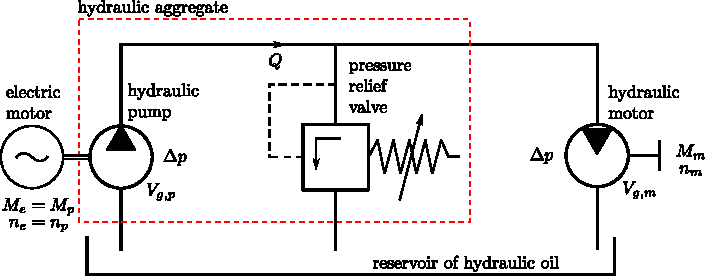
\includegraphics[height=5cm]{PositiveDisplacementPumps/Figures/Sizing_Of_System_With_Motor.pdf}
	\caption{Block diagram of the simplest hydraulic system with a single hydraulic motor driven by a single hydraulic aggregate.}
	\label{fig:hydraulic_aggregate_with_motor}
\end{figure}

As a specific example, let us consider a task where a machine have to be operated with a revolution number of $n_m=1500\,\mathrm{rpm}$ by a hydraulic motor. To maintain the rotation, a torque of $M_m=100\,\mathrm{Nm}$ is required. The first step is to make an initial guess for the system pressure of the underlying hydraulic system; for instance, let $\Delta p^*=200\,\mathrm{bar}$ (later, it can be adjusted if necessary). According to Eq.\,\eqref{power_balance_of_positive_displacement_machines} in Sec.\,\ref{sec:basic_characteristics_of_positive_displacement_machines}, the required geometric volume of the hydraulic motor can be estimated:
%
\begin{equation}
V_{g,m}^* = \frac{2 \pi M_m}{\Delta p^*} \frac{\eta_{v,m}}{\eta_{hm,m}} = 3.142 \cdot 10^{-5}\,\mathrm{m^3} = 31.4\,\mathrm{cm^3},
\end{equation}
%
where $\eta_{v,m}=1$ and $\eta_{hm,m}=1$ are the volumetric and hydromechanical efficiency, respectively. For simplicity, they considered unity in this specific example (no losses). For simple hydraulic devices, the geometric volume (sometimes called displacement in catalogues) is fixed; and for a family of products, there is a specific size series. It is to be stressed that there are products with adjustable geometric volume; however, these devices are much more expensive due to their complicated constructions. Using a Bosch Rexroth external gear motor from the AZMG series (fixed displacement to reduce costs), the closest geometric volume is
%
\begin{equation}
V_{g,m}=32\,\mathrm{cm^3}.
\end{equation}
%
The system pressure difference has to be adjusted according to the real geometric volume:
%
\begin{equation}
\Delta p = \frac{2 \pi M_m}{V_{g,m}} \frac{\eta_{v,m}}{\eta_{hm,m}} = 196.35\,\mathrm{bar}.
\end{equation}
%
The maximum operating pressure for the selected hydraulic motor is $p_{max}=250\,\mathrm{bar}$ that is much higher than our operation pressure $p=\Delta p + p_0$. Therefore, no additional adjustment of the system pressure is needed. If the value of $\Delta p$ had been higher than $p_{max}$, the geometric volume should be recalculated preferably with a lower initial guess of the system pressure. Parenthetically, the pressure difference can be calculated as $\Delta p=p-p_0$, where $p$ is the absolute system pressure (at the inlet of the hydraulic motor) and $p_0$ is the ambient pressure (at the outlet of the hydraulic motor). Since $p_0 \approx 1\,\mathrm{bar}$ (the reservoir is usually open to the environment) and $p \gg p_0$, the pressure difference is $\Delta p \approx p$. In addition, the maximum revolution number of the hydraulic motor is $2800\,\mathrm{rpm}$; thus, the device meets the requirements.

The volume flow rate necessary to drive the motor at a revolution number of $n_m=1500\,\mathrm{rpm}$ is
%
\begin{equation}
Q_r = \frac{V_{g,m} n_m}{\eta_{v,m}} = 8 \cdot 10^{-4}\,\mathrm{\frac{m^3}{s}} = 48\,\mathrm{\frac{dm^3}{min}} = 48\,\mathrm{\frac{l}{min}}.
\end{equation}
%
The next task in the sizing is the proper selection of a pump that can provide the required flow rate $Q_r$. Assume that the electric motor that drives the pump has a revolution number of $n_e=n_p=3000\,\mathrm{rpm}$. Keep in mind that revolution numbers of the available electric motors can be selected from a limited number of standard values (unless an expensive frequency converter is applied). The geometric volume of the hydraulic pump must be greater than
%
\begin{equation}
V_{g,p}^{min} = \frac{Q_r}{n_p \eta_{v,p}} = 1.6 \cdot 10^{-5}\,\mathrm{m^3} = 16\,\mathrm{cm^3}.
\end{equation}
%
Due to safety reasons and the always presented volumetric efficiency (considered $\eta_{v,p}=1$ here for simplicity), the actual geometric volume must definitely be bigger than the value of $V_{g,p}^{min}$. Using a Bosch Rexroth external gear pump from the AZPG series, a pump with a geometric volume of
%
\begin{equation}
V_{g,p} = 22\,\mathrm{cm^3}
\end{equation}
%
is selected. The maximum revolution number is $3000\,\mathrm{rpm}$ for this geometric volume; thus, the pump meets the requirements as well. Observe that due to the larger geometric volume than the required, the actual volume flow rate the pump provides is
%
\begin{equation}
Q_p = V_{g,p} n_p \eta_{v,p} = 66\,\mathrm{\frac{dm^3}{min}} = 66\,\mathrm{\frac{l}{min}},
\end{equation}
%
which is much larger than $Q_r=48\,\mathrm{l/min}$ needs for the hydraulic motor. Therefore, a suitable control technique has to be employed to reduce the volume flow rate passing through the hydraulic motor, for details see Sec.\,\ref{sec:control_techniques_of_hydraulic_systems}.

The torque needs to drive the pump is approximately
%
\begin{equation}
M_e = M_p = \frac{\Delta p V_{g,p}}{2 \pi} \frac{\eta_{v,p}}{\eta_{hm,p}} = 50.9\,\mathrm{Nm}.
\end{equation}
%
The hydromechanical efficiency of the pump is also considered unity ($\eta_{hm,p}=1$). Based on the values of $n_e$ and $M_e$, a suitable electric motor can also be selected. This is beyond the scope of the present investigation. Keep in mind, however, that the torque the electric motor can provide must be somewhat greater than the minimum required $M_e$ (for safety reasons). The final task is to set the opening pressure of the pressure relief valve of the hydraulic aggregate. Let it be $20\%$ above the system pressure $\Delta p$ to ensure robust operation: $\Delta p_{set} \approx 240\,\mathrm{bar}$.

%------------------------------------------------
\subsection{A hydraulic system with cylinder} \label{sec:hydraulic_system_with_cylinder}
The second major application of hydraulic systems when a hydraulic aggregate drives a hydraulic cylinder. The block diagram of such a configuration is depicted in Fig.\,\ref{fig:hydraulic_aggregate_with_cylinder}, which is similar to that of shown in Fig.\,\ref{fig:hydraulic_aggregate_with_motor}. The only difference is the replacement of the hydraulic motor with a cylinder. A hydraulic cylinder (also called a \textit{linear} hydraulic motor) is a mechanical actuator that is used to give a unidirectional force through a unidirectional stroke. It consists of a cylinder barrel, in which a piston connected to a piston rod moves back and forth. The barrel is closed on one end by the bottom of the cylinder (also called the cap) and the other end by the cylinder head (also called the gland) where the piston rod comes out of the cylinder. 

The direction of the displacement of the cylinder is managed by a 4-way, 3 position direction valve. Port $P$ is the supply (system pressure), port $R$ is the return to the reservoir, $A$ and $B$ are general-purpose system ports. The centre is the closed position where both system ports are closed, and the supply port is connected to the return port; that is, this is an idle operation where the position of the piston is fixed (even if there is heavy load $F$ on the piston rod) due to the incompressibility of the hydraulic oil. If the direction valve switched upward, the supply port $P$ and the system port $B$ are connected, and the piston of the cylinder moves upward as well. Meanwhile, the return port $R$ is connected to the system port $A$; thus, the hydraulic oil can be released to the reservoir from the upper part of the cylinder allowing the displacement of the piston. In contrast, if the direction valve switched downward, the supply port $P$ is connected to the system port $A$ and the hydraulic aggregate drives the piston in the downward direction. Observe that in this case, the return port $R$ is connected to the system port $B$ releasing the hydraulic oil back to the reservoir from the lower part of the hydraulic cylinder. Strictly speaking, a direction valve is necessary to control the position of the piston in the cylinder.

\begin{figure}[ht!]
	\centering
		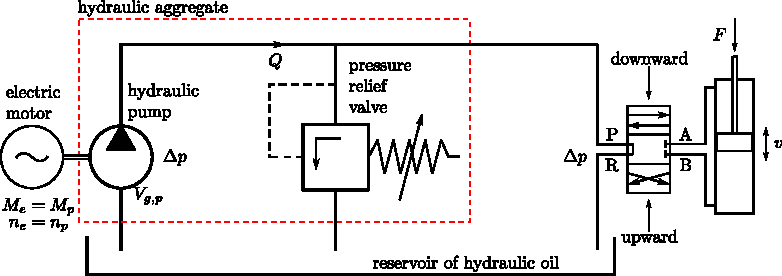
\includegraphics[height=5cm]{PositiveDisplacementPumps/Figures/Sizing_Of_System_With_Cylinder.pdf}
	\caption{Block diagram of the simplest hydraulic system with a single hydraulic cylinder driven by a single hydraulic aggregate.}
	\label{fig:hydraulic_aggregate_with_cylinder}
\end{figure}

Let us continue the discussion with a specific example. Consider a weight of $m=5\,\mathrm{t}$ that the cylinder have to elevate with a speed of $v=0.5\,\mathrm{m/s}$. The diameter of the piston of the cylinder is $D=63\,\mathrm{mm}$. In this case, the pressure difference need to elevate the weight is
%
\begin{equation}
\Delta p = \frac{F}{A} = \frac{mg}{D^2 \pi /4} = 157.35\,\mathrm{bar},
\end{equation}
%
where $g=9.81\,\mathrm{m/s^2}$ is gravitational acceleration. The required volume flow rate can be calculated via the task-specific requirements for the speed $v$ of the elevation:
%
\begin{equation}
Q_r = A v = \frac{D^2 \pi}{4} v = 0.0016\,\mathrm{\frac{m^3}{s}} = 93.5\,\mathrm{\frac{dm^3}{min}} = 93.5\,\mathrm{\frac{l}{min}}.
\end{equation}
%
The rest of the sizing procedure is the same as in the case of the previous example. Assuming that the driving electric motor has a revolution number of $n_e=n_p=1500\,\mathrm{rpm}$, the minimum required geometric volume of the hydraulic pump is
%
\begin{equation}
V_{g,p}^{min} = \frac{Q_r}{n_p \eta_{v,p}} = 6.2 \cdot 10^{-5}\,\mathrm{m^3} = 62.3\,\mathrm{cm^3}.
\end{equation}
%
The volumetric efficiency of the pump is again considered unity ($\eta_{v,p}=1$). Choosing a Bosch Rexroth external gear pump from the AZPG series, the closest possible option is $63\,\mathrm{cm^3}$. However, for safety reasons (due to the volumetric efficiencies), the selected geometric volume is
%
\begin{equation}
V_{g,p} = 70\,\mathrm{cm^3}.
\end{equation}
%
Again, because of the larger $V_{g,p}$ that necessary, the actual volume flow rate is
%
\begin{equation}
Q_p = V_{g,p} n_p \eta_{v,p} = 0.0018\,\mathrm{\frac{m^3}{s}} = 105\,\mathrm{\frac{dm^3}{min}} = 105\,\mathrm{\frac{l}{min}},
\end{equation}
%
which must be controlled down to $Q_r=93.5\,\mathrm{l/min}$, see Sec.\,\ref{sec:control_techniques_of_hydraulic_systems}.

The torque needs to drive the pump is approximately
%
\begin{equation}
M_e = M_p = \frac{\Delta p V_{g,p}}{2 \pi} \frac{\eta_{v,p}}{\eta_{hm,p}} = 175.3\,\mathrm{Nm},
\end{equation}
%
where, as usual, $\eta_{hm,p}=1$ for simplicity. Again, based on the values of $n_e$ and $M_e$, a suitable electric motor can also be selected. Again, this is beyond the scope of the present investigation, and keep in mind again that the torque the electric motor can provide must be somewhat higher than the minimum required $M_e$ (for safety reasons). The opening pressure of the pressure relief valve of the hydraulic aggregate is set $20\%$ above the system pressure $\Delta p$ to ensure robust operation: $\Delta p_{set} \approx 190\,\mathrm{bar}$.

%------------------------------------------------
\subsection{Control techniques of hydraulic systems} \label{sec:control_techniques_of_hydraulic_systems}
In Secs.\ref{sec:hydraulic_system_with_hydraulic_motor} and \ref{sec:hydraulic_system_with_cylinder}, it is shown that with basic hydraulic elements, the required flow rate for the hydraulic motor or the cylinder can rarely be set precisely. Usually, a bigger hydraulic pump is chosen in order to ensure the needed volume flow rate. However, the difference between the flow rates of the pump $Q_p$ and the required $Q=Q_m=Q_c$ for the motor or the cylinder must be treated somehow. The simplest technique, discussed in this section in more details, is to install and adjust a throttle so that a surplus of the flow rate is released back to the reservoir through the pressure relief valve or a bypass pipe. This ``trick'' is simple and cheap, but the losses are usually very high. In many industrial hydraulic applications; however, such an additional loss plays an insignificant role. For instance, in cases where the hydraulic motor/cylinder used only a few times in a day for few minutes/seconds (e.g., in a car repair workshop to elevate cars before service).

If the overall efficiency of the hydraulic system is important, more sophisticated control techniques are available. Naturally, these solutions are much more expensive. One option is to choose an electric motor with a frequency converter and regulate the revolution number $n_e=n_p$ of the electric motor and the pump. In this way, the flow rate of the pump can be set precisely. Another option is to select a pump or hydraulic motor with variable displacement (variable geometric volume $V_{g,p}$ and/or $V_{g,m}$). By changing the geometric volume, the produced (pump) or required (motor) volume flow rate can be adjusted to the needs. Such devices have a complex internal structure making them very expensive. Note that the variable geometric volume cannot be applied to hydraulic cylinders. The aforementioned sophisticated techniques are beyond the scope of the present topic.

%-----------------------
\subsubsection{Throttle valve in parallel connection}
The first control technique discussed in this section is the application of a throttle connected in parallel to the hydraulic aggregate and to the hydraulic motor, see the block diagram in Fig.\,\ref{fig:control_of_hydraulic_system_parallel_throttle}. If the throttle is totally open, all the flow rate produced by the pump flows back to the reservoir through the throttle as this is the route with the least resistance. Therefore, the volume flow rate of the pump and the throttle is equal ($Q_p=Q_{th}$). In contrast, when the throttle is completely closed, all the flow rate produced by the pump is delivered to the hydraulic motor: $Q_p=Q_m$. In any other intermediate cases, the volume flow rate produced by the pump is distributed between the throttle and the motor; namely, $Q_p=Q_{th}+Q_{m}$. The main idea is to set the opening of the throttle so that the volume flow rate of the motor becomes precisely the required one ($Q_m=Q_r$), and the surplus ($Q_{th}=Q_p-Q_r$) flows down through the throttle directly to the reservoir.

\begin{figure}[ht!]
	\centering
		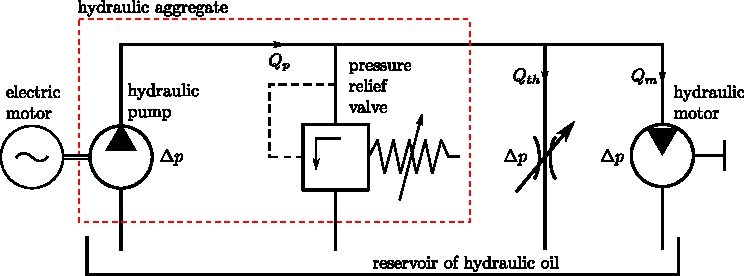
\includegraphics[height=5cm]{PositiveDisplacementPumps/Figures/Control_Of_Hydraulic_System_Parallel_Throttle.pdf}
	\caption{Block diagram of the control of a hydraulic system with a throttle connected in parallel.}
	\label{fig:control_of_hydraulic_system_parallel_throttle}
\end{figure}

In order to give an insight how much power is lost at the throttle, let us represent the control mechanism in a $(\Delta p, Q)$ diagram shown in Fig.\,\ref{fig:energy_efficiency_parallel_throttle}. The calculated values of the different quantities are also depicted for the case discussed in Sec.\,\ref{sec:hydraulic_system_with_hydraulic_motor}. First of all, the thick red curve is the characteristic curve of the hydraulic aggregate composed by a nearly vertical (pump) and horizontal (pressure relief valve) lines, for details the reader is referred to Sec.\,\ref{sec:pressure_relief_valve}. Since the operating system pressure $\Delta p=196.35\,\mathrm{bar}$ is below the opening pressure of the pressure relief valve $\Delta p_{set}=240\,\mathrm{bar}$, the operation point of the hydraulic aggregate (black dot) lies on the vertical part of the red curve. Therefore, this is the operation point of the pump as well. Keep in mind that the pressure difference $\Delta p$ is identical for the pump, motor and throttle, see also Fig.\,\ref{fig:control_of_hydraulic_system_parallel_throttle}. If the throttle is properly tuned (for instance by hand until the required revolution number of the motor is achieved), the volume flow rate of the motor must be
%
\begin{equation}
Q_m = Q_r = 48\,\mathrm{\frac{l}{min}},
\end{equation}
%
and the rest of the flow rate produced by the pump is flown back to the reservoir through the throttle:
%
\begin{equation}
Q_{th} = Q_p - Q_m = 66\,\mathrm{\frac{l}{min}} - 48\,\mathrm{\frac{l}{min}} = 18\,\mathrm{\frac{l}{min}}.
\end{equation}
%
Keep in mind also, that due to the slightly inclined characteristic curve of the pump (the nearly vertical part of the red curve in Fig.\,\ref{fig:energy_efficiency_parallel_throttle}), the actual flow rate of the pump can be a slightly bit smaller than the theoretically calculated $66\,\mathrm{l/min}$ in Sec.\,\ref{sec:hydraulic_system_with_hydraulic_motor}. However, this causes no safety issue as the pump is oversized, and it provides a good estimates for the energetic calculations.

\begin{figure}[ht!]
	\centering
		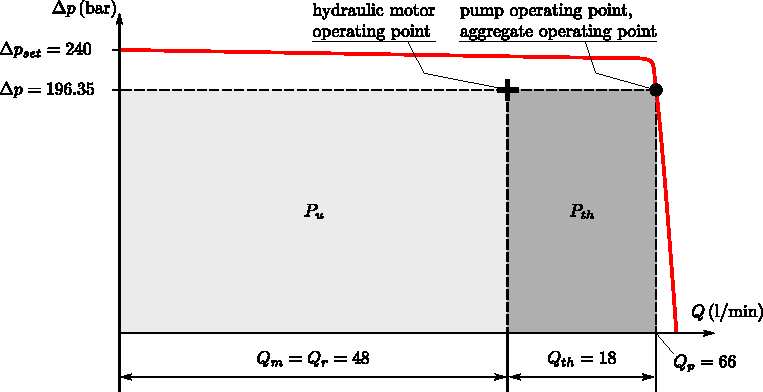
\includegraphics[height=7cm]{PositiveDisplacementPumps/Figures/Energy_Efficiency_Parallel_Throttle.pdf}
	\caption{Energetic consideration of the control of a hydraulic system with a parallel throttle.}
	\label{fig:energy_efficiency_parallel_throttle}
\end{figure}

As the hydraulic power is the multiplication of the pressure difference $\Delta p$ and the volume flow rate $Q$, the power dissipated at the throttle $P_{th}$ and the useful power that ``arrives'' to the motor $P_u$ can be represented as a rectangular area in Fig.\,\ref{fig:control_of_hydraulic_system_parallel_throttle}. Precisely, the useful power is
%
\begin{equation}
P_u = Q_m \Delta p = 8 \cdot 10^{-4}\,\mathrm{\frac{m^3}{s}} \cdot 196.35 \cdot 10^5\,\mathrm{Pa} = 15708\,\mathrm{W} = 15.7\,\mathrm{kW},
\end{equation}
%
the power loss at the throttle is
%
\begin{equation}
P_{th} = Q_{th} \Delta p = 3 \cdot 10^{-4}\,\mathrm{\frac{m^3}{s}} \cdot 196.35 \cdot 10^5\,\mathrm{Pa} = 5890\,\mathrm{W} = 5.9\,\mathrm{kW},
\end{equation}
%
and finally, the total input power introduced by the pump is
%
\begin{equation}
P_i = P_p = Q_p \Delta p = (Q_m+Q_{th}) \Delta p = P_u + P_{th} = 21599\,\mathrm{W} = 21.6\,\mathrm{kW}.
\end{equation}
%
Observe that in this control technique, $27.3\%$ of the total input power is dissipated at the throttle. In the next subsection, a different (but similarly simple) technique is introduced and compared its efficiency with the above-described method.

%-----------------------
\subsubsection{Throttle valve in series connection}
The second control technique discussed in this section is the application of a throttle connected in series to the hydraulic aggregate and the hydraulic motor, see the block diagram in Fig.\,\ref{fig:control_of_hydraulic_system_serial_throttle}. If the throttle is totally open, all the flow rate produced by the pump flows through the hydraulic motor (as if there were no throttle installed). In this case, the volume flow rate of the pump and the hydraulic motor is equal, which is higher then the required ($Q_p=Q_m>Q_r$). During an initial range of the closure of the throttle, no change in the flow rate is observed (up to a specific closure). Only the pressure difference the pump has to produce increases, since it is the sum of the pressure drop at the throttle $\Delta p_{th}$ and at the hydraulic motor $\Delta p_m$:
%
\begin{equation} \label{pressure_distrubution_in_serial_throttle}
\Delta p_p = \Delta p_{th} + \Delta p_m.
\end{equation}
%
If the throttle closed enough, the pressure difference of the pump reaches the opening pressure of the pressure relief valve; that is, $\Delta p_p=\Delta p_{set}$. By closing the throttle further, the pressure relief valve opens even more, and an increasing amount of flow rate $Q_{prv}$ is released back to the reservoir bypassing the hydraulic motor. Due to the conservation of mass, the flow rate of the pump is
%
\begin{equation}
Q_p = Q_{prv} + Q_m,
\end{equation}
%
meaning that a decreased amount of flow rate passing through the hydraulic motor (decreased by $Q_{prv}$). When the throttle is totally closed, the pressure relief valve is totally open, and all the flow rate flow through the pressure relief valve ($Q_p=Q_{prv}$, $Q_m=0$). The main aim in this control technique is to close the throttle so much that the flow rate of the motor becomes the required: $Q_m=Q_r$. For this, the flow rate released back to the reservoir through the pressure relief valve is $Q_{prv}=Q_p-Q_r$. Again, the precise closure of the throttle is hard to determined by paper and pencil; it is set usually by continuously monitoring the revolution number of the motor, and stop the closing if the required revolution number (proportional to the flow rate) is reached.

\begin{figure}[ht!]
	\centering
		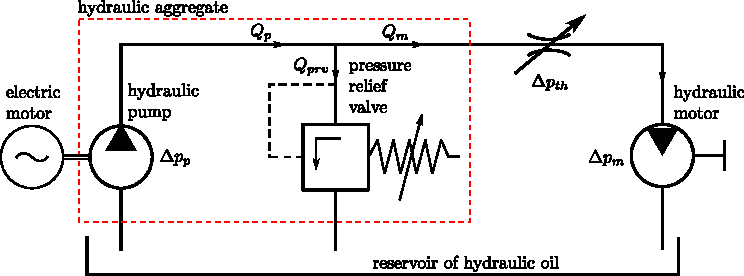
\includegraphics[height=5cm]{PositiveDisplacementPumps/Figures/Control_Of_Hydraulic_System_Serial_Throttle.pdf}
	\caption{Block diagram of the control of a hydraulic system with a serially connected throttle.}
	\label{fig:control_of_hydraulic_system_serial_throttle}
\end{figure}

Similarly, as in case of the control technique of the parallel throttle, represent the control mechanism in a $(\Delta p, Q)$ diagram shown in Fig.\,\ref{fig:energy_efficiency_serial_throttle}. Again, the values of the quantities calculated in Sec.\,\ref{sec:hydraulic_system_with_hydraulic_motor} are also depicted. The characteristic curve of the hydraulic aggregate (solid red curve) is the same as in the case of Fig.\,\ref{fig:energy_efficiency_parallel_throttle}. The extension of the characteristic curve of the pump is depicted by the red dashed line. The throttle has to be closed so much that the flow rate of the hydraulic aggregate, which flows through the throttle and the hydraulic motor as well, must be
%
\begin{equation}
Q_m = Q_{th} = Q_r = 48\,\mathrm{\frac{l}{min}}.
\end{equation}
%
Therefore, the operating point of the hydraulic aggregate (red dot) must lie on the red curve at the required flow rate of $48\,\mathrm{l/min}$. At this point, there is an elevated pressure difference close to the opening pressure of the pressure relief valve. As the characteristic curve of the pressure relief valve (nearly horizontal line) is slightly inclined, the ``working'' pressure difference is slightly below the opening pressure $\Delta p_{set}$. However, this difference is usually marginal, and for simplicity, we assume that the working pressure difference of the hydraulic aggregate and the pump is equal to the opening pressure of the pressure relief valve:
%
\begin{equation}
\Delta p_p = \Delta p_{ha} = \Delta p_{set} \approx 240,\,\mathrm{bar},
\end{equation}
%
where the subscript $ha$ stands for hydraulic aggregate. The pressure difference produced by the pump serves to satisfy the need of the pressure drop at the hydraulic motor and the pressure loss at the throttle, see Eq.\,\eqref{pressure_distrubution_in_serial_throttle}. The pressure drop at the motor is $\Delta p_m = 196.35\,\mathrm{bar}$ need to produce the required torque $M_m$ for the rotation. Thus, the pressure loss at the throttle can be calculated as
%
\begin{equation}
\Delta p_{th} = \Delta p_{set} - \Delta p_m \approx 43.65,\,\mathrm{bar}.
\end{equation}
%
The pressure difference $\Delta p_m$ and the flow rate $Q_m=Q_r$ determines the operating point of the hydraulic motor marked by the black cross in Fig.\,\ref{fig:energy_efficiency_serial_throttle}. The operation point of the pump (back dot) must lie on the characteristic curve of the pump itself instead of the characteristic curve of the hydraulic aggregate. That is why the characteristic curve of the pump is extended (see the red dashed line). Observe that the black dot does not lie on the solid red curve anymore, although the deviation from it is very small. Again, the actual flow rate of the pump is changing slightly as a function of the pressure difference; thus, it is not exactly equal to $66\,\mathrm{l/min}$ calculated in Sec.\,\ref{sec:hydraulic_system_with_hydraulic_motor}. The difference, however, is marginal, and it is a reasonable assumption to neglect this effect.

\begin{figure}[ht!]
	\centering
		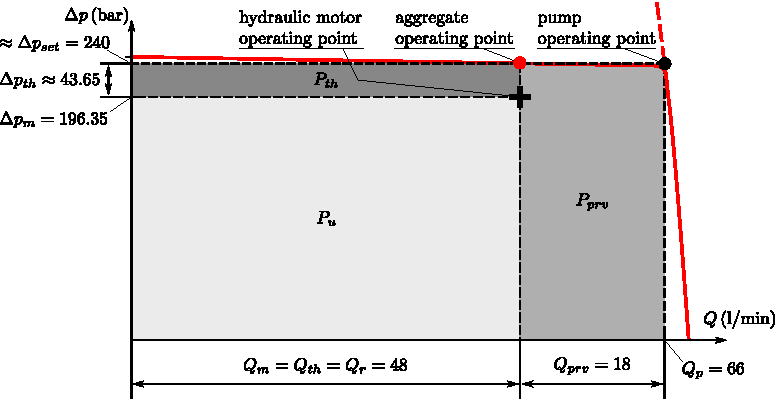
\includegraphics[height=7cm]{PositiveDisplacementPumps/Figures/Energy_Efficiency_Serial_Throttle.pdf}
	\caption{Energetic consideration of the control of a hydraulic system with a serial throttle.}
	\label{fig:energy_efficiency_serial_throttle}
\end{figure}

The hydraulic power can be calculated in a similar way as in case of the previous example; namely, multiply the pressure difference dropped at a specific device with the corresponding volume flow rate. The hydraulic power of the motor, pressure relief valve and the throttle is marked by the grey shaded area labelled with $P_m=P_u$, $P_{prv}$ and $P_{th}$, respectively, in Fig.\,\ref{fig:energy_efficiency_serial_throttle}. Numerically, the hydraulic power of the motor that is the useful power is the same as in the case of the parallel throttle control:
%
\begin{equation}
P_u = Q_m \Delta p_m = 8 \cdot 10^{-4}\,\mathrm{\frac{m^3}{s}} \cdot 196.35 \cdot 10^5\,\mathrm{Pa} = 15708\,\mathrm{W} = 15.7\,\mathrm{kW}.
\end{equation}
%
The power loss at the throttle is
%
\begin{equation}
P_{th} = Q_{th} \Delta p_{th} = 8 \cdot 10^{-4}\,\mathrm{\frac{m^3}{s}} \cdot 43.65 \cdot 10^5\,\mathrm{Pa} = 3492\,\mathrm{W} = 3.5\,\mathrm{kW}.
\end{equation}
%
Observe how the operating condition of the throttle is different from the parallel technique, which is emphasized also by the quite distinct shaded regions for $P_{th}$ in Figs.\,\ref{fig:energy_efficiency_parallel_throttle} and \ref{fig:energy_efficiency_serial_throttle}. Note that although the power loss is less than in the parallel connection, the hydraulic power at the pressure relief valve is also considered as a loss (it has no contribution to the useful power):
%
\begin{equation}
P_{prv} = Q_{prv} \Delta p_{set} = 3 \cdot 10^{-4}\,\mathrm{\frac{m^3}{s}} \cdot 240 \cdot 10^5\,\mathrm{Pa} = 7200\,\mathrm{W} = 7.2\,\mathrm{kW}.
\end{equation}
%
Therefore, the total power loss is
%
\begin{equation}
P_{l}=P_{th}+P_{prv}=10.7\,\mathrm{kW}.
\end{equation}
%
Finally, the input power introduced by the pump is
%
\begin{equation}
\begin{split}
P_i &= P_p = Q_p \Delta p_{set} = (Q_m+Q_{prv}) \Delta p_{set} = Q_m (\Delta p_m+\Delta p_{th}) + P_{prv} \\
    &= P_u + P_{th} + P_{prv} = 26400\,\mathrm{W} = 26.4\,\mathrm{kW}.
\end{split}
\end{equation}
%
In this control technique, $40.5\%$ of the total input power is dissipated at the throttle and the pressure relief valve; this is much higher than the parallel throttle case ($27.3\%$). The total input power required by the pump is also higher due to the elevated operation pressure difference from $\Delta p=196.35\,\mathrm{bar}$ (see also Fig.\,\ref{fig:energy_efficiency_parallel_throttle}) to $\Delta p_{set}=240\,\mathrm{bar}$. One can conclude that the serial throttle technique has more substantial losses as the hydraulic aggregate works at the opening pressure of the pressure relief valve rather than the designed value $\Delta p = \Delta p_m < \Delta p_{set}$. However, as mentioned previously, using a simple throttle (either serial or parallel) to regulate the flow rate of the hydraulic motor is useful in situations where the losses play a minor role during the operation, see the discussion in the introduction of Sec.\,\ref{sec:control_techniques_of_hydraulic_systems}.

%------------------------------------------------
% TODO???
%\input{pressure_vessel_sizing.tex}


% In gear pumps the liquid is trapped by the opening between the gear teeth of two identical gears and the chasing of the pump on the suction side. On the pressure side the fluid is squeezed out when the teeth of the two gears are rotated against each other. The motor provides the drive for one gear.

% The lobe pumps operates similar to the gear pump, but with two lobes driven by external timing gears. The lobes do not make contact.

% Progressive cavity pumps consist of a metal rotor rotating within an elastomer-lined or elastic stator. When the rotor turns progressive chambers from suction end to discharge end are formed between the rotor and stator, moving the fluid. 


\section{Problems}

\noindent {\bf Problem \thesection.\theprob}\stepcounter{prob}

Calculate the hydraulic power of the double-acting piston pump, which delivers water from an open-surface tank into a closed one with $500[kPa]$ gauge pressure (i.e. relative pressure) located $50[m]$ above the suction tank. Diameter of the piston is $D=120[mm]$, the stroke is $150[mm]$ and the driving motor runs at $120[rpm]$.

\emph{Solution:} 

$Q_{mean}=2 \times A_{piston} \times s \times n=2\times \frac{0.12^2 \pi}{4} \times 0.15 \times \frac{120}{60} =6.78 \times 10^{-3} [\frac{m^3}{s}]$

$\Delta p=p_{tank,abs.}-p_0\,+\,\rho g H=p_{tank,rel.}\,+\,\rho g H=991[kPa]$

$P=Q \Delta p=6.72[kW]$

%%%%%%%%%%%%%%%%%%%%%%%%%%%%%%%%%%%%%%%%%%%%%%%%%%%%

\vspace{1cm}
\noindent {\bf Problem \thesection.\theprob}\stepcounter{prob}

The characteristic curve of a gear pump is $Q[dm^3/min]=11.93-0.0043 \Delta p [bar]$. The volumetric efficiency at $35 bar$ pressure difference is $92\%$. Find the volume flow rate and the geometric volume! The shaft speed is $80 rev/min$. How large is the driving torque if the pump efficiency is $85\%$? (Solution: $Q=11.78\,dm^3/min$, $V_g = 160\,cm^3$, $M = 96.5\,Nm$)

%%%%%%%%%%%%%%%%%%%%%%%%%%%%%%%%%%%%%%%%%%%%%%%%%%%%

\vspace{1cm}
\noindent {\bf Problem \thesection.\theprob}\stepcounter{prob}

The piston diameter of a hydraulic cylinder is $50 mm$. An $800 kg$ load is lifted by the piston rod of $20 mm$ diameter with $12 m/min$ velocity. How large must be the flow rate $Q$ of the gear pump rotating with $n = 960/min$ speed if its volumetric efficiency is $92\%$? Find the geometric volume of the pump and the pressure rise produced by it! Find the power $P$ and the torque $M$ of the driving motor! The pump efficiency is $74\%$. Prepare a sketch of the gear pump showing the rotation direction of the shafts, intake and delivery ports! How large will be $P’$, $M$, $Q’$ if the rotor speed is $n’ = 1440/min$? (Solution: $Q_g = 21.5\,dm^3/min$, $V_g = 22.4\,cm^3$, $\Delta p = 47.6\,bar$, $P=2.12\,kW$, $M=21.1\,Nm$, $P_{1440}=3.18\,kW$, $Q_{1440} = 32.25\,dm^3/min$, $M_{1440}=21.1\,Nm$)

%%%%%%%%%%%%%%%%%%%%%%%%%%%%%%%%%%%%%%%%%%%%%%%%%%%%

\vspace{1cm}
\noindent {\bf Problem \thesection.\theprob}\stepcounter{prob}

The piston diameter of a vertical hydraulic cylinder is supporting a mass of $700 kg$. It may not be lowered faster than $64 mm/s$. The cylinder diameter is $50 mm$, the piston rod diameter is $28 mm$. The pump delivery curve is $Q [liter/min] = 8.6-0.0467 \Delta p[bar]$. The hydraulic oil of $970 kg/m^3$ density leaves the cylinder through a throttle valve. The discharge coefficient of this valve is $\mu=0.7$. Find the valve area at the maximal opening! Find the maximum of the useful power of the pump! 

Solution:

\begin{wrapfigure}{R}{0.4\textwidth}
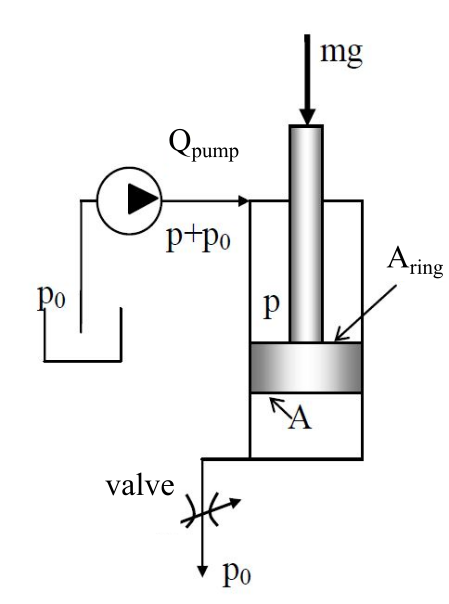
\includegraphics[width=0.4\textwidth]{Problem_solving/figs/cylinder-problem.png}
\end{wrapfigure}

The two areas:
\begin{align*}
A_{ring} = \frac{\pi}{4} (D^2-d^2) = 0.001348~\mathrm{m^2}\\
A = \frac{\pi}{4} D^2 = 0.001964~\mathrm{m^2}.
\end{align*}

Newton's law:
%\begin{align*}
%A(p_0+\Delta p_{valve}) = A_{ring}p + mg = A_{ring}(p_0 + \Delta p) + mg + A_{piston}p_0 = Ap_0 + A_{ring} \Delta p + mg.
%\end{align*}
\begin{multline*}
A(p_0+\Delta p_{valve}) = A_{ring}p + mg = \\
A_{ring}(p_0 + \Delta p) + mg + A_{piston}p_0 = Ap_0 + A_{ring} \Delta p + mg.
\end{multline*}

Continuity equation for the upper part of the cylinder:
\begin{align*}
Q_{pump} = A_{ring}v = 0.001347~\mathrm{m^2}\cdot 0.064~\frac{\mathrm{m}}{\mathrm{s}} = 5.176~\frac{\mathrm{dm^3}}{\mathrm{min}}.
\end{align*}

Pressure from the performance curve of the pump:
\begin{align*}
\Delta p = \frac{8.6-Q_{pump}}{0.0467} = \frac{8.6-5.176}{0.0467} = 73.3~\mathrm{bar}.
\end{align*}

Continuity equation for the valve:
\begin{align*}
Q_{valve} = Av = 0.001964~\mathrm{m^2}\cdot 0.064~\frac{\mathrm{m}}{\mathrm{s}} = 7.54~\frac{\mathrm{dm^3}}{\mathrm{min}}.
\end{align*}

Bernoulli's equation for the valve: 
\begin{align*}
Q_{valve} = \mu A_{valve}\sqrt{\frac{2}{\rho_{oil}}\Delta p_{valve}}.
\end{align*}

Rearranging Newton's law yields
\begin{align*}
\Delta p_{valve} = \frac{A_{ring}\Delta p + mg}{A} = \frac{0.001348\cdot 7.33\cdot 10^6 + 700\cdot 9.81}{0.001964} = 85.27~\mathrm{bar}, 
\end{align*}
and finally,
\begin{align*}
A_{valve} = \frac{Q_{valve}}{\mu \sqrt{\frac{2}{\rho_{oil}}\Delta p_{valve}}} = \frac{0.0001257}{0.7\cdot \sqrt{\frac{2}{970}\cdot 85.27\cdot 10^5}} = 1.354~\mathrm{mm}.
\end{align*}

The useful power of the pump is
\begin{align*}
P_{p,u}=Q_{pump}\Delta p_{pump} = (8.6-0.0467 \Delta p)\Delta p.
\end{align*}

The criterion for the local maximum is $\frac{\mathrm{d}P_{p,u}}{\mathrm{d}\Delta p} = 8.6-2\cdot 0.0467\cdot \Delta p_{opt} = 0 \rightarrow \Delta p_{opt} = 92.1~\mathrm{bar}$. At this operating point, $Q_{opt}=4.3~\frac{1}{\mathrm{min}}$, and $P_{p,u,max} = 660~\mathrm{W}$.


\clearpage

%\section{Problems}

%\noindent {\bf Problem \thesection.\theprob}\stepcounter{prob}

%Calculate the hydraulic power of the double-acting piston pump, which delivers water from an open-surface tank into a closed one with $500[kPa]$ gauge pressure (i.e. relative pressure) located $50[m]$ above the suction tank. Diameter of the piston is $D=120[mm]$, the stroke is $150[mm]$ and the driving motor runs at $120[rpm]$.

%\emph{Solution:} 

%\begin{itemize}
%\item $Q_{mean}=2 \cdot A_{piston} \cdot s \cdot n=2\cdot \frac{0.12^2 \pi}{4} \cdot 0.15 \cdot \frac{120}{60} =6.78 \cdot 10^{-3} [\frac{m^3}{s}]$
%\item $\Delta p=p_{tank,abs.}-p_0\,+\,\rho g H=p_{tank,rel.}\,+\,\rho g H=991[kPa]$
%\item $P=Q \Delta p=6.72[kW]$
%\end{itemize}
